\documentclass[11pt,a4paper,twoside]{article}

% ---------------- IMPORTE -----------------------------
\usepackage[german]{babel}
\usepackage{blindtext}
\usepackage{color}
\usepackage{graphicx}
\usepackage{fancyhdr}
\usepackage[left=25mm, right=25mm, top=25mm, bottom=33mm]{geometry} % Seitenränder
\usepackage{parskip}
\usepackage{tabularx,colortbl}
\usepackage{wrapfig}
\usepackage{epstopdf}
\usepackage{minted}
%\usepackage[font={small,it}]{caption}
%\usepackage{colortbl}
%\usepackage{listings}
\usepackage[utf8]{inputenc}
\usepackage{tocloft}
\usepackage{setspace}
\usepackage{tcolorbox}
\usepackage{subfig}
\usepackage{prettyref}
\usepackage{enumitem}
\usepackage{bold-extra}
\usepackage{ragged2e}
\usepackage{pstricks}
\usepackage{pifont}
\usepackage[abs]{overpic}
\usepackage{hyperref}

% --------------- Klickbare Links --------------------------
\hypersetup{
    colorlinks=true,
    linktoc=all,
    linkcolor=black,
}

% --------------- Querverweis --------------------------
\newrefformat{fig}{Abbildung \ref{#1}}
\newrefformat{sec}{\ref{#1}}

% --------------- Common-Settings ----------------------
\epstopdfsetup{outdir=./}
\setlength{\abovecaptionskip}{5px}
\setlength{\belowcaptionskip}{0pt}
\setlength{\extrarowheight}{4pt}
\setlength{\cftfigindent}{0px}
\captionsetup{justification=centering}

% --------------- CODE-Beispiele -----------------------
\tcbuselibrary{minted,skins}
\newtcblisting{javacode}[1][]{
  listing engine=minted,
  colframe=white,
  listing only,
  minted style=colorful,
  minted language=java,
  minted options={linenos=true,fontsize=\footnotesize,numbersep=2mm,texcl=false,#1},
  left=5mm,enhanced,
  top=0mm, bottom=0mm,
  overlay={\begin{tcbclipinterior}\fill[black!15] (frame.south west)
            rectangle ([xshift=5mm]frame.north west);\end{tcbclipinterior}}
}

\tcbset{arc=0mm}

% --------------- ADITO-spezifische Farben -------------
\definecolor{ADITO_RED}{rgb}{0.93,0.09,0.32}

% --------------- Neuer Spaltentyp ---------------------
\newcolumntype{P}[1]{>{\centering\arraybackslash}p{#1}} %zentriert eine Spalte mit fester Breite

% ---------------- Seitenzahlen rechts + Logo ----------
\pagestyle{fancy}
\fancyhf{}

\fancyhead[L]{\textbf{\textsc{Shortcut-Editor}} \\ Implementierung eines Editors zur Bearbeitung von Tastaturkürzeln}
\fancyhead[R]{\vspace{-5mm}\includegraphics[height=0.045\textheight]{../graphic/images/logo/Logo}}
\fancyfoot[LE,RO]{\thepage}
\fancyfoot[LO,RE]{\copyright\ Korbinian Mifka}

\renewcommand{\headrulewidth}{1pt}
\renewcommand{\footrulewidth}{1pt}
% ------------------------------------------------------
% ------------------------------------------------------
\begin{document}
\begin{titlepage}

\begin{center}
\includegraphics[scale=0.25]{../img/LogoIHK.pdf}\\[1ex]
\Large{Abschlussprüfung Sommer 2018}\\[3ex]

\Large{Fachinformatiker für Anwendungsentwicklung}\\
\LARGE{Dokumentation zur betrieblichen Projektarbeit}\\[4ex]

\huge{\textbf{Shortcut-Editor}}\\[1.5ex]
\Large{\textbf{Implementierung eines Editors zur Bearbeitung von Tastaturkürzeln}}\\[4ex]

\normalsize
\begin{tabularx}{0.54\textwidth}{rl}
Abgabetermin: & 18.05.2018 \\
Projektverantwortlicher: & Robert Loipfinger\\
\end{tabularx}
\\[3em]

\textbf{Prüfungsbewerber:}\\
Korbinian Mifka\\

\vfill


\includegraphics[scale=0.7]{../img/ADITO_Logo}\\[2ex]
\textbf{Ausbildungsbetrieb:}\\
ADITO Software GmbH\\
Konrad Zuse Str. 4\\
84144 Geisenhausen\\[5em]
\end{center}

\small
\noindent
Dieses Werk einschließlich seiner Teile ist \textbf{urheberrechtlich geschützt}.
Jede Verwertung außerhalb der engen Grenzen des Urheberrechtgesetzes ist ohne
Zustimmung des Autors unzulässig und strafbar. Das gilt insbesondere für
Vervielfältigungen, Übersetzungen, Mikroverfilmungen sowie die Einspeicherung
und Verarbeitung in elektronischen Systemen.

\end{titlepage}
\pagenumbering{gobble}
\tableofcontents
\thispagestyle{fancy}
\newpage

\pagenumbering{arabic}
\setcounter{page}{1}
\section{Einleitung}

\begin{wrapfigure}[12]{r}[0cm]{180px}
	\vspace{-12px}
	\centering
	\includegraphics[width=1\linewidth]{../graphic/images/firma/Firmengebaude}
	\caption{Firmengbäude}
	\label{fig:firmengebaude}
\end{wrapfigure}

Die folgende Projektdokumentation beschreibt den Ablauf des IHK-Abschlussprojektes, welche der Autor im Rahmen der Ausbildung zum Fachinformatiker Fachrichtung Anwendungsentwicklung durchgeführt hat. Ausbildungsbetrieb ist die ADITO Software GmbH, ein Hersteller für hochflexible Business-, CRM- und xRM-Software mit Sitz in Geisenhausen. Das inhabergeführte Unternehmen bietet Entwicklung, Vertrieb, Projektierung und Service aus einer Hand. Kunden von ADITO kommen aus den unterschiedlichsten Branchen. Neben namhaften mittelständischen Unternehmen, zum Beispiel Ravensburger, Erlus oder Birco, gehören auch große Organisationen wie die WWK Versicherungsgruppe oder die Bundesagentur für Arbeit zu ihren Referenzen.

Die Mitarbeiterzahl des Unternehmens ist insbesondere in den letzten Jahren stark gewachsen. Im Jahr 2018 hat ADITO die Grenze von 100 Mitarbeitern überschritten. Um dafür genügend Raum zu bieten, wurde im gleichen Jahr ein neues Firmengebäude (\autoref{fig:firmengebaude}) errichtet.

\subsection{Beschreibung}
 
In der neuesten Version des xRM-Systems ADITO5 wurde eine neue Clientvariante entwickelt. Nun ist es möglich neben dem konventionellen Java Swing Client, einen Webclient bzw. Browserclient einzusetzen. Dieser bietet einige Vorteile. Beispielsweise ist keine Installation notwendig und die Nutzung ist auf allen Geräten mit Webbrowsern (PC, Tablet und Smartphone) möglich. 

Mit einem Webclient gehen allerdings auch einige Herausforderungen einher. So auch bei der Vergabe von Tastaturkürzeln. Browser behalten es sich vor, einige Shortcuts für eigene Aktionen zu reservieren und so nicht für die eigentliche Webanwendung zur Verfügung zu stellen. Beispiele für solche Shortcuts sind \emph{Strg + P} für Drucken oder \emph{Strg + F} für Suchen. Der Überblick über die Verwendbarkeit von Tastaturkürzeln geht schnell verloren, da diese in jeder Browser-Betriebssystem-Permutation variieren kann.

Im Rahmen dieser Arbeit soll eine Möglichkeit geschaffen werden, bei der Vergabe von Shortcuts innerhalb der hauseigenen xRM-Entwicklungsumgebung (ADITO5 Designer) Unterstützung zu bieten.

\subsection{Ziel}

Um den Entwicklern unserer xRM-Software die Vergabe von Shortcuts zu erleichtern, soll ein spezieller Shortcut-Editor erstellt werden. Dieser muss die Eingabe und Bearbeitung von Shortcuts ermöglichen und bei der Wahl des passenden Tastenkürzels zuarbeiten.

Warnungen im Editor verdeutlichen, dass der eingegebene Shortcut zu Problemen auf einem bestimmten Browser führen kann. Damit der Entwickler feststellen kann, warum ein Shortcut problematisch ist, sollen weitere Informationen angezeigt werden. Diese können beispielsweise angeben, bei welchem Browser bzw. welcher Version das Tastaturkürzel bereits verwendet wird.

\subsection{Umfeld}

Durchgeführt wird das Projekt in der Entwicklungsabteilung, welche auch für die Umsetzung von ADITO5 zuständig war. Die Notwendigkeit des Editors wurde im Zuge der Weiterentwicklung festgestellt. Dadurch kann man die Abteilung Entwicklung selbst als Auftraggeber ihres eigenen Projekts ansehen.

Die Implementierung des Editors wird in der objektorientierten Programmiersprache Java und mithilfe der Entwicklungsumgebung IntelliJ IDEA durchgeführt. Als Framework für die grafische Benutzeroberfläche dient das Java-Swing-Framework.

\subsection{Begründung}

Da gewährleistet werden soll, dass vergebene Tastenkürzel auf allen relevanten Browsern funktionieren, muss dem Entwickler bei der Wahl eines passenden Shortcuts immer klar sein, ob dieser von den entsprechenden Browsern unterstützt wird. Da jeder Browser andere Shortcuts vorbelegt und diese sich je nach Betriebssystem wieder unterscheiden können, ist eine manuelle Überprüfung durch den Projektierer unzumutbar. So müsste dieser auf jedem Betriebssystem alle relevanten Browser testen. Ein derartig enormer Aufwand und die mögliche Fehlvergabe von Tastenkombinationen können durch die technische Assistenz mittels des genannten Editors vermieden werden.

\subsection{Schnittstellen}
\label{schnittstellen} 

Um herauszufinden, welche Shortcuts die verschiedenen Browser auf unterschiedlichen Betriebssystemen verwenden, wurde außerhalb dieser Abschlussarbeit eine Testanwendung implementiert. Diese kann auf verschiedenen Betriebssystemen (z. B. Windows, Linux und MacOS) ausgeführt werden und testet alle möglichen Shortcut-Kombinationen für die verbreitetsten Browser (z. B. Chrome, Firefox oder Safari). Das Ergebnis dieser Tests wird in Form von XML-Dateien gespeichert (Beispiel siehe Anhang \ref{xml}). Für jede Browser-Betriebssystem-Kombination existiert eine eigene Datei, in welcher alle problembehafteten Shortcuts verzeichnet sind.

Damit die in den Dateien enthaltenen Informationen dem Benutzer dargestellt werden können, muss der Editor das Einlesen und Verarbeiten von XML-Strukturen beherrschen. Hierfür kommt das hauseigene \emph{Propertly} Framework zum Einsatz. Dieses kümmert sich um sämtliche XML-spezifische Arbeiten und ermöglicht so eine komfortable Nutzung.

Die über den Editor ausgewählten Shortcuts werden Aktionen zugeordnet, welche bereits im ADITO5 Designer implementiert wurden. Zudem existieren sogenannte Entitys, welche Dateneinheiten darstellen und eben genannte Aktionen besitzen können. Beispielsweise könnte ein Entity \glqq Firma\grqq\xspace existieren, welches wiederum die Aktion \glqq Mitarbeiter hinzufügen\grqq\xspace besitzt. Dieser Aktion könnte nun ein Shortcut zugewiesen werden z. B. \emph{Strg + Einfg}.


\subsection{Abgrenzung}

Aufgrund des beschränkten Projektumfangs ist das Einbinden des Editors in den bestehenden ADITO5 Designer nicht Bestandteil der Projektarbeit.






\newpage
\section{Projektplanung}

\subsection{Entwicklungsprozess}

Um das Projekt realisieren zu können, musste sich für einen geeigneten Entwicklungsprozess entschieden werden. Dieser gibt die Vorgehensweise vor, welche der Umsetzung zu Grunde liegt. Für dieses Projekt wurde vom Autor das Wasserfallmodell gewählt. Dabei wird die Umsetzung auf 5 Phasen aufgeteilt (siehe \autoref{fig:wasserfallmodell}): Die Ermittlung der Anforderungen, die Erstellung eines Entwurfs, die Implementierung und am Ende die Überprüfung und Wartung der erstellten Software. Dieses Modell bietet sich für diese Arbeit an, da die Anforderungen an den Editor klar definiert sind und sich während der Umsetzungsphase nicht ändern.

\begin{figure}[H]
	\centering
	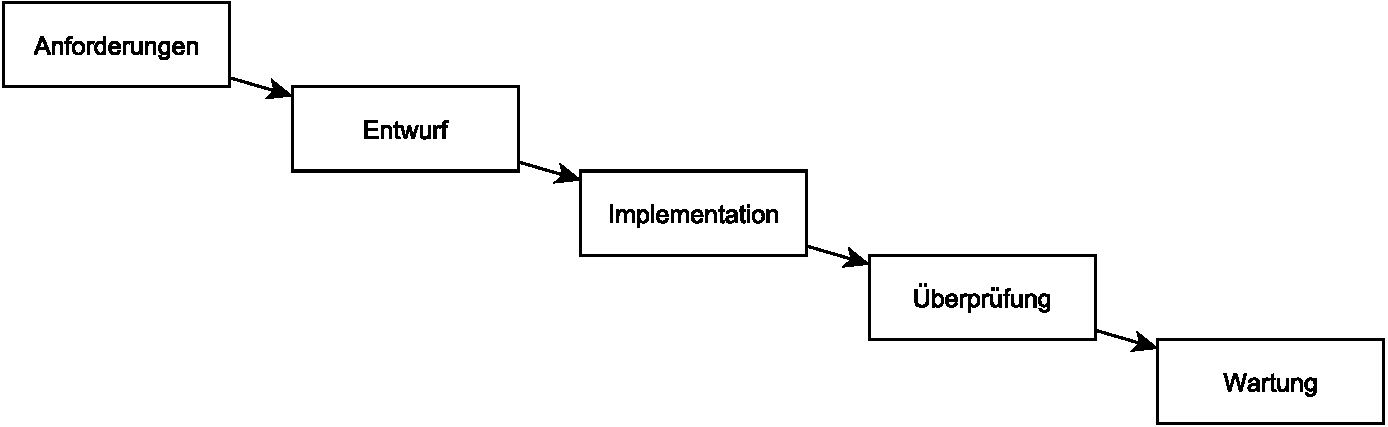
\includegraphics[height=78px]{../graphic/diagrams/SD_Wasserfallmodell/Wasserfallmodell}
	\caption{Wasserfallmodell}
	\label{fig:wasserfallmodell}
\end{figure}

\subsection{Projektphasen}
\label{Projektphasen}

Zur Realisierung des Abschlussprojekts standen insgesamt 70 Stunden zur Verfügung. Diese Zeit wurde vor Projektbeginn auf verschiedene Phasen verteilt, die während der Durchführung durchlaufen werden. Diese Zeitplanung der Hauptphasen lässt sich aus \autoref{fig:grobeZeit} entnehmen.

\begin{figure}[H] 
	\begin{center}
		\begin{tabularx}{0.90\textwidth}{X|P{50px}|P{50px}}
			\hline \rowcolor{ADITO_RED} \textcolor{white}{\textbf{Vorgang}} & \textcolor{white}{\textbf{Geplante Zeit in h}} 	\\
			\hline
			1. Analysephase													& 3 	\\ 
			
			2. Entwurfsphase						 						& 15 	\\
			
			3. Implementierungsphase										& 40	\\
			
			4. Testphase													& 2 	\\
			5. Dokumentationserstellung										& 10 	\\ 
			\hline 
			& 70 \\
		\end{tabularx}
	\end{center}
	\caption{Grobe Zeitplanung} 
	\label{fig:grobeZeit}
\end{figure}

\subsection{Ressourcenplanung}

Im Zuge der Ressourcenplanung wurde eine Übersicht (siehe Anhang \ref{ressources}) erstellt. Diese enthält sämtliche Ressourcen, welche innerhalb der Durchführung des Projekts eingesetzt wurden. Dabei handelt es sich sowohl um Hard- und Softwareressourcen als auch um Personal. Zur Minimierung der Projektkosten wurde bevorzugt kostenfreie Software verwendet. War dies nicht möglich, so wurde Software eingesetzt, für welche die ADITO Software GmbH bereits Lizenzen besaß.



\newpage
\section{Projektanalyse}

Im Rahmen der Projektanalyse wird der IST-Zustand ermittelt und dem SOLL-Zustand gegenübergestellt

\begin{wrapfigure}[6]{r}[0cm]{180px}
	\vspace{-40px}
	\centering
	\includegraphics[width=140px]{../img/Alter-Editor.PNG}
	\caption{Bestehender Editor}
	\label{fig:existEditor}
\end{wrapfigure}

\subsection{Ist-Analyse}

Aktuell existiert bereits ein Editor zur Eingabe von Shortcuts (siehe \autoref{fig:existEditor}). Dieser ist allerdings sehr einfach aufgebaut und beschränkt sich auf die Eingabe eines Shortcuts per Tastatur. Außerdem ist es nicht möglich Warnungen anzuzeigen oder zwischen bestehenden Shortcuts zu navigieren.

\subsection{Soll-Analyse}



\vfill

\begin{figure}[H] 
	\subfigure{\includegraphics[width=0.5\textwidth]{../img/ux/2-ShortCutEditor-Eingabe.jpg}} 
	\subfigure{\includegraphics[width=0.5\textwidth]{../img/ux/4-ShortCut-Info.jpg}}
	\caption{UX-Entwürfe} 
\end{figure}

\newpage
\section{Entwurfsphase}

\subsection{Architekturdesign}
\label{Architekturdesign}

Als passendes Entwurfsmuster für den Shortcut Editor hat sich das Model View Presenter (MVP)-Architekturmuster herausgestellt. Dieses ist nicht ganz so verbreitet wie das bekanntere Model View Controller (MVC)-Muster, ist diesem aber sehr ähnlich. Der eigendliche Unterschied zwischen MVP und MVC liegt darin, dass bei MVC die View neben dem Controller auch mit dem Model kommuniziert und dieses somit kennen muss. Bei MVP ist die View völlig unabhängig vom Model und nur der Presenter kommuniziert mit ihr (siehe \autoref{fig:modelview}). Der Autor hat sich für das MVP-Entwurfsmuster entschieden, da damit die View auch ohne Model verwendet werden kann und es denkbar ist, das diese Möglichkeit in Zukunft benötigt wird.

\begin{figure}[H] 
	\subfloat{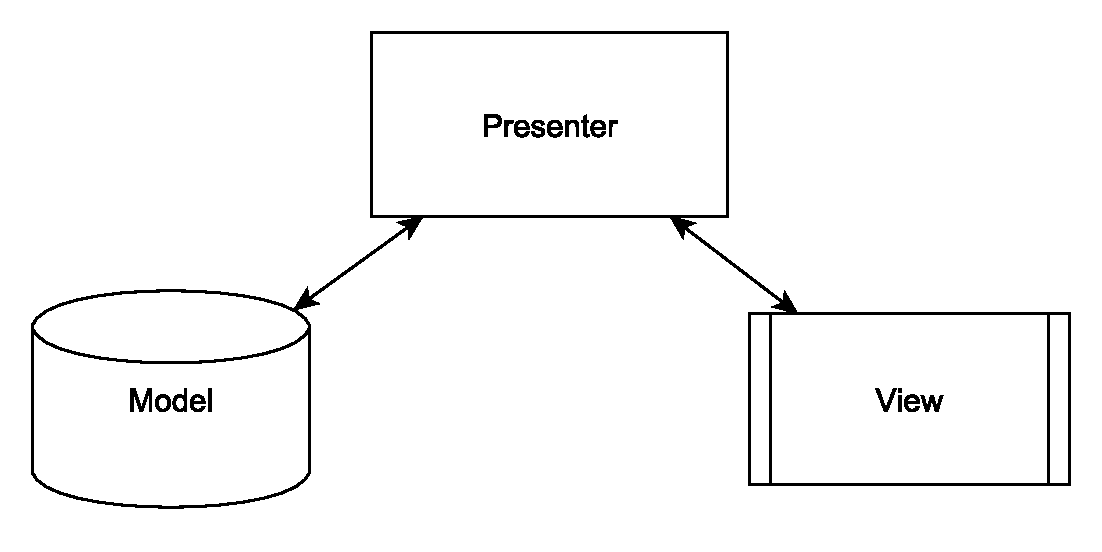
\includegraphics[width=0.5\textwidth-5px]{../graphic/diagrams/ModelViewPresenter/ModelViewPresenter}}
	\hfill 
	\subfloat{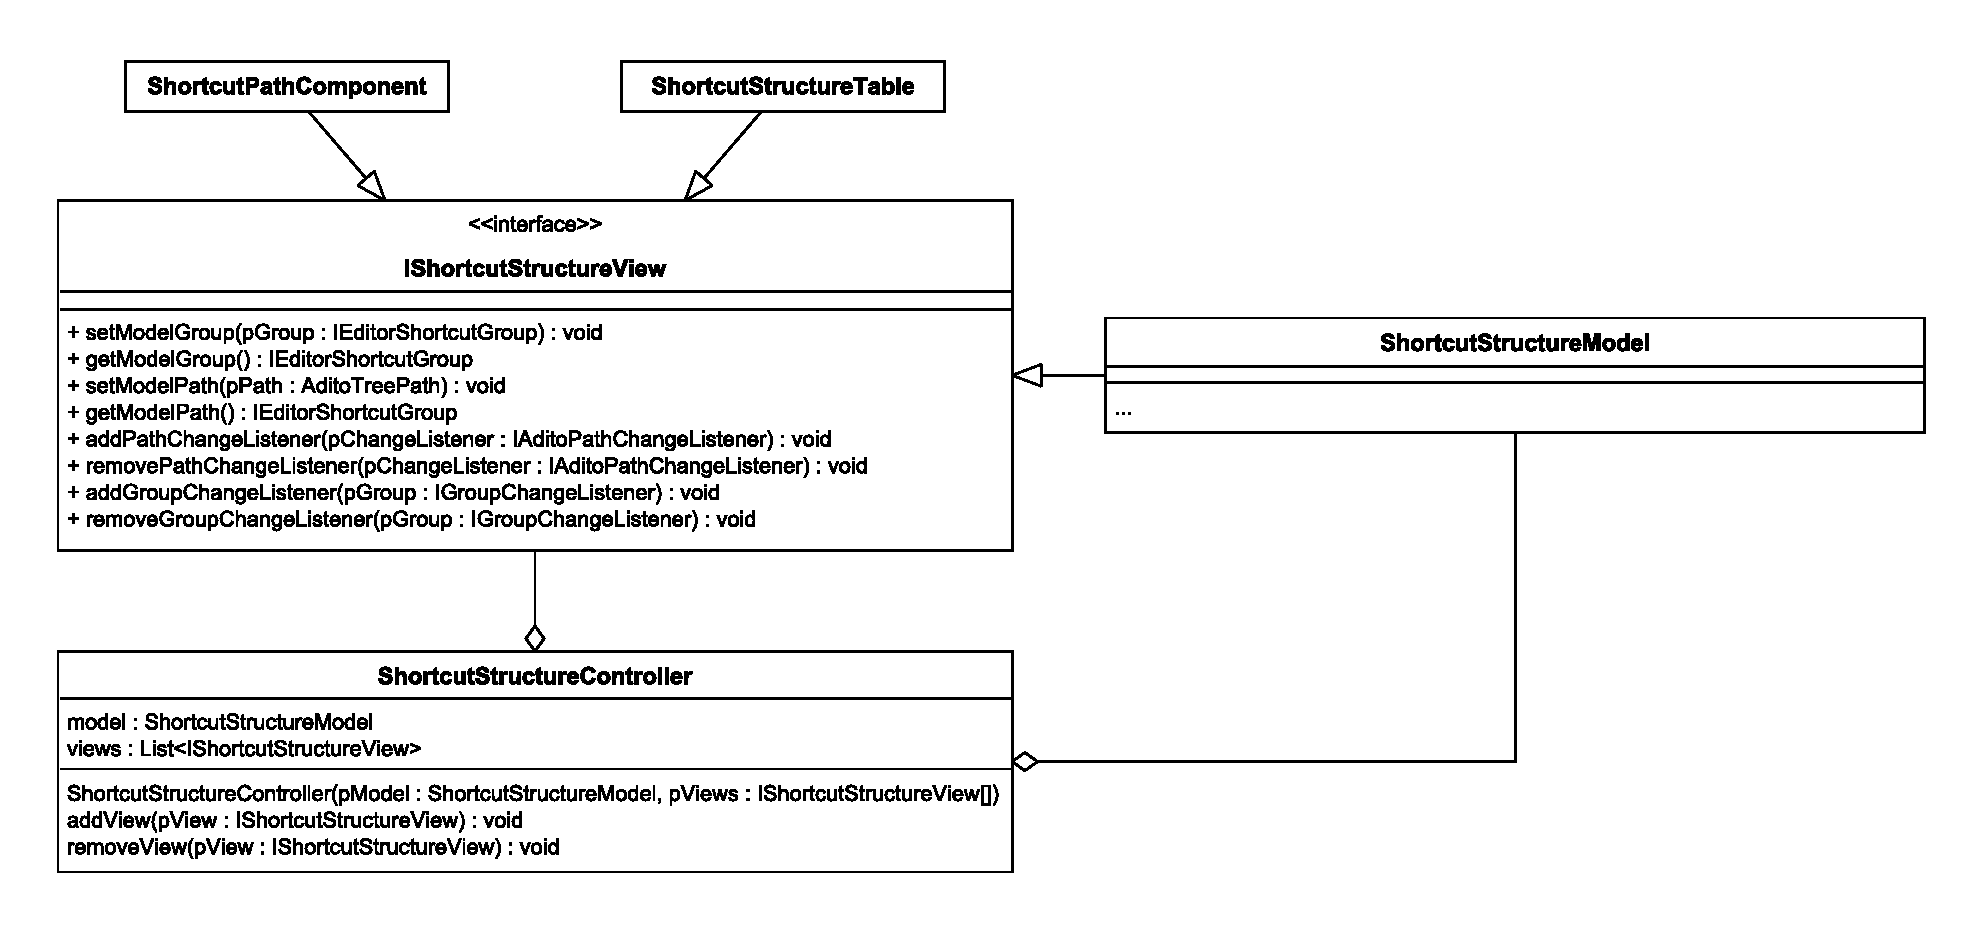
\includegraphics[width=0.5\textwidth-5px]{../graphic/diagrams/ModelViewController/ModelViewController}}
	\caption{Model View Presenter vs. Model View Controller} 
	\label{fig:modelview}
\end{figure}

Bei MVP lässt sich jede Komponente der Software einem der drei Bestandteile - Model, View oder Presenter - zuordnen. Jeder dieser Teile hat einen eigenen Aufgabenbereich, der von denen der anderen weitestgehend unabhängig ist. Im Model werden alle Daten gehalten und zur Verfügung gestellt. Die View kümmert sich um die grafische Darstellung und der Presenter stellt das Bindeglied zwischen der View und dem Model dar. Verändern sich beispielsweiße die Werte in der View, so kümmert sich der Presenter darum, dass diese Wertänderung im Model ebenso stattfindet und andersherum. Der Presenter hält somit die View -- oder auch mehrere Views untereinander -- und das Model auf dem gleichen stand. Die lose Kopplung der einzelnen Komponenten erhöht die Wiederverwendbarkeit und Austauschbarkeit. Man könnte beispielsweise die Benutzeroberfläche austauschen, ohne das Model anpassen zu müssen. Außerdem können die einzelnen Komponenten durch die strikte Trennung einfacher getestet, gewartet und flexibel erweitert werden. Diese Vorteile sprechen ebenso für eine Verwendung von MVP.

\vfill

Im Sinne der Wiederverwendbarkeit, werden auch alle GUI-Komponenten des Shortcut Editors völlig seperat voneinander und unabhängig vom Editor implementiert. Dadurch kann gewährleistet werden, keine unnötigen Abhängigkeiten zu editorspezifischen Teilen aufzubauen. So ist die Benutzung von Komponenten auch an anderen Stellen in der Software ohne weiteren Aufwand möglich.

\vfill

Wie im Abschnitt \ref{schnittstellen} bereits erwähnt, wird für das Lesen der Testergebnis XML-Dateien das hauseigene Propertly Framework verwendet. Dieses Tool stellt Funktionalitäten zum Lesen und Schreiben von XML zur Verfügung. Außerdem kümmert es sich eigendständig um die Konvertierung von Datentypen. Dadurch kommt der Autor bei der Implementierung nicht mit XML spezifischen Arbeiten in Berührung und kann sich auf den eigentlichen Editor konzentrieren.

\newpage

\subsection{Benutzeroberfläche}
\label{ui}

Für das Design des User Interfaces (UI) wurden von einem UX-Designer der ADITO Software GmbH Entwürfe angefertigt (siehe \autoref{fig:uxDesigns}). Im Designentwurf wird ersichtlich, welche Komponenten verwendet werden müssen, um alle angeforderten Informationen darzustellen und wie diese aussehen und angeordet zu sein haben, um die bedarfsgerechte Bedienung zu ermöglichen. Nachfolgend werden die Bestandteile des Editors näher erläutert:

\ding{192} \textbf{Breadcrumb:} Diese Komponente ist in der Lage einen Pfad darzustellen und diesen zu bearbeiten. In diesem Fall besteht sie aus beliebig vielen ComboBoxen, um an jeder Stelle des Pfads einen anderen Knoten auswählen zu können. Diese Komponente dient zum Einen als Orientierungshilfe, um jederzeit feststellen zu können, für welche Aktion der Shortcut gesetzt wird. Zum Anderen ist damit eine intuitive Navigation durch alle Aktionen möglich.

\ding{193} \textbf{Shortcut-Field:} Hierbei handelt es sich um eine Komponente, welche die Darstellung und Bearbeitung von Shortcuts ermöglicht. Die Eingabe und Editierung des Tastaturkürzels kann nur bei fokusiertem Zustand erfolgen. Demnach wechselt die Komponente bei Fokusierung in den Bearbeitungsmodus und verlässt diesen, sobald eine andere Komponente den Fokus erlangt.

\ding{194} \textbf{Check-Button:} Dieses GUI-Element kann selektiert werden und stellt neben einem Icon ein Häckchen- oder Kreuzsymbol dar. Somit kann die Komponente visualisieren, bei welchem Browser bzw. Betriebssystem der Shortcut Probleme bereiten kann (Kreuz) und wo dieser unbedenklich ist (Häckchen). Außerdem dient sie dem Benutzer zur Auswahl eines Elements, um davon mehr Informationen zu erhalten (Im Entwurf werden beispielhaft für Google Chrome und macOS detailierte Informationen angezeigt).

\ding{195} \textbf{Shortcut-Tag:} Ein Shortcut-Tag dient zur Darstellung einer Tastenkombination und bietet die Möglichkeit sich mittles eines Kreuz-Buttons selber zu entfernen.

\ding{196} \textbf{TreeTable:} Zur Darstellung der zugrundeliegenden Baumstruktur wird zur Visualisierung aller Aktionen eine Kombination aus Tree und Tabelle verwendet. Sie dient -- wie die \textbf{Breadcrumb} -- der Navigation und bietet zudem einen Überblick über alle vorhandenen Shortcuts.

\ding{197} \textbf{Accordion:} Ist ein \textbf{Check-Button} selektiert, so wird eine Accordion-Komponente angezeigt, welche detailierte Informationen zu den Testergebnissen bietet. Um nur relevante Daten anzuzeigen, besteht die Möglichkeit einige Sektionen durch Klicken auf den Header einzuklappen.

\begin{figure}[H] 
	\begin{overpic}[width=1\linewidth,unit=1px]%
		{../graphic/images/ux/Kombination}
		\put(75,175){\ding{182}}
		\put(134,163){\ding{183}}
		\put(217,149){\ding{184}}
		\put(34,149){\ding{184}}
		\put(375,80){\ding{184}}
		
		\put(185,110){\ding{185}}
		\put(185,101){\ding{185}}
		
		\put(185,82){\ding{185}}
		\put(185,73){\ding{185}}
		
		\put(185,56){\ding{185}}
		
		\put(185,37){\ding{185}}
		\put(185,27){\ding{185}}
		
		\put(110,79){\ding{186}}
		\put(280,137){\ding{187}}
		\put(280,68){\ding{187}}
		
	\end{overpic}

	\caption{Designentwurf des UX-Designers}
	\label{fig:uxDesigns}
\end{figure}

\newpage

\subsection{Datenmodell für Entitäten und Aktionen}
\label{DatenmodellFunc}

\begin{wrapfigure}[17]{r}[0cm]{200px}
	\vspace{-12px}
	\centering
	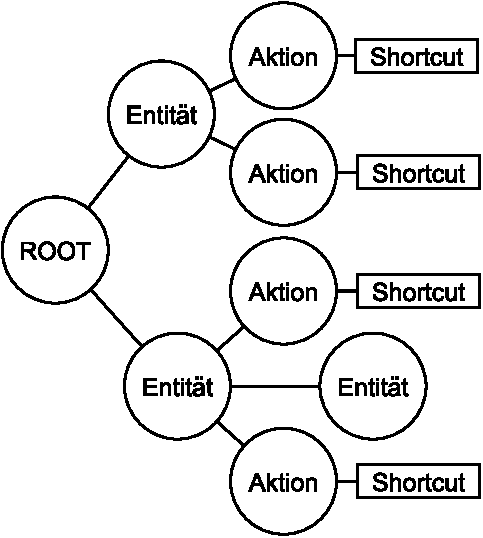
\includegraphics[width=200px]{../graphic/diagrams/Baumstruktur_Functions/Baumstruktur}
	\caption{Baumstruktur für Entitäten und Funktionen}
	\label{fig:baumstruktur_Func}
\end{wrapfigure}

Wie sich im Designentwurf (\autoref{fig:uxDesigns}) -- aufgrund der TreeTable -- schon erahnen lässt, sollen die Entitäten und deren Aktionen als Baumstruktur aufgebaut werden. Jede Aktion stellt einen Endknoten (Blatt) dar und soll genau einen Shortcut besitzen können. Entitäten hingegen ist es nur erlaubt, Aktionen und weitere Entitäten aufzunehmen (siehe \autoref{fig:baumstruktur_Func}). Da es sich um eine Baumstruktur handelt, kann man ausschließen, dass sich eine Entität selbst als Kind hält.

Um diese Struktur im Editor abbilden zu können, wurde ein Datenmodell entworfen, welches den Anforderungen entspricht. Zur Erläuterung des Models ist im Folgenden ein schematisches UML Klassendiagramm abgebildet, welches den Grundaufbau und die Beziehungen zwischen den Elementen verdeutlicht (\autoref{fig:baumstrukturUML_Func}).

\vfill

Zentraler Bestandteil des Datenmodells ist das Interface \textbf{IEditorShortcutNode}. Dieses kann neben einem eigenen Namen auch seine Kinder zurückgeben. Diese sind ebenfalls vom Typ \textbf{IEditorShortcutNode}. Damit kann grundsätzlich schon eine Baumstrukturen aufgebaut werden. Allerdings ist durch \textbf{IEditorShortcutNode} nur die Abbildung der Bestandteile \textbf{ROOT} und \textbf{Entity} aus \autoref{fig:baumstruktur_Func} möglich, da noch kein Tastenkürzel gehalten werden kann.

\vfill

\begin{figure}[H]
	\vspace{20px}
	\centering
	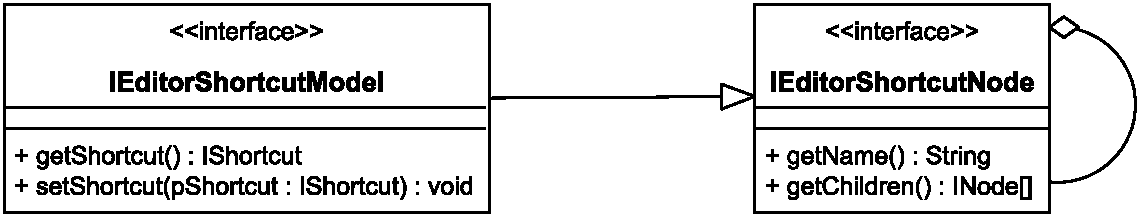
\includegraphics[height=57px]{../graphic/diagrams/CD_Baumstruktur_Functions/Baumstruktur}
	\caption{Datenmodell für Entitäten und Aktionen}
	\label{fig:baumstrukturUML_Func}
\end{figure}

\vfill

Um auch eine Aktion im Modell abbilden zu können, existiert das Interface \textbf{IEditorShortcutModel}. Dieses erbt von \textbf{IEditorShortcutNode} und stellt somit einen vollwertigen Knoten dar, welcher bei der Methode \textbf{getChildren()} zurückgegeben werden kann. Über die Methoden \textbf{setShortcut(...)} kann eine Tastenkombination gesetzt und über \textbf{getShortcut()} ausgelesen werden. Da diese Methoden nur die Zuweisung von einem einzigen Shortcut zulassen, ist sichergestellt, dass eine Aktion nur ein Tastenkürzel besitzen kann. Aufgrund der Tatsache, dass \textbf{IEditorShortcutModel} einen Endknoten (Blatt) darstellt und somit keine Kinder hat, liefert die geerbte Methode \textbf{getChildren()} ein leeres Array. Für die Iteration durch den Baum ist es programmatisch konfortabler und effizienter, wenn jeder Knoten die Methode \textbf{getChildren()} besitzt, da andernfalls unnötige Abfragen stattfinden müssen.

Über diese Konstellation lässt sich die Baumstruktur der Aktionen und deren Shortcuts den Anforderungen entsprechend abbilden.

\newpage

\subsection{Datenmodell für Browsertestergebnisse}
\label{DatenmodellBrow}

\begin{wrapfigure}[9]{l}[0cm]{165px}
	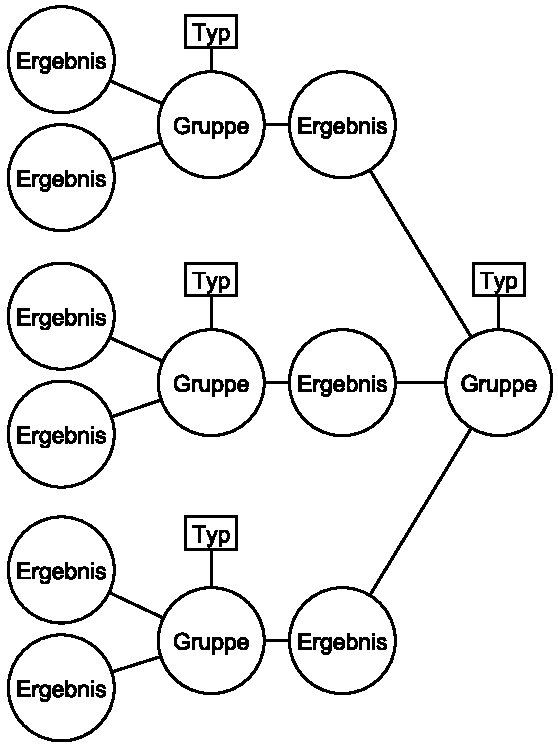
\includegraphics[width=165px]{../graphic/diagrams/Baumstruktur_Results/Baumstruktur}
	\caption{Baumstruktur für Browsertestergebnisse}
	\label{fig:baumstruktur_Result}
\end{wrapfigure}

Auch die Browserergebnisse werden als Baumstruktur gehalten. Allerdings ergiebt sich hierbei eine neue Anforderung. Betrachtet man den Designentwurf, so stellt man fest, dass eine Gruppe von Testergebnissen immer eine Typenbezeichnung hat (Im Entwurf haben die Gruppen den Typ \glqq Browser\grqq\xspace oder \glqq Betriebssystem\grqq). In \autoref{fig:baumstrukturUML_Results} ist ein UML-Klassendiagramm eines Datenmodells abgebildet, welches den Anforderungen zum Halten von Browsertestergebnissen gerecht wird.

\begin{figure}[H]
	\flushright
	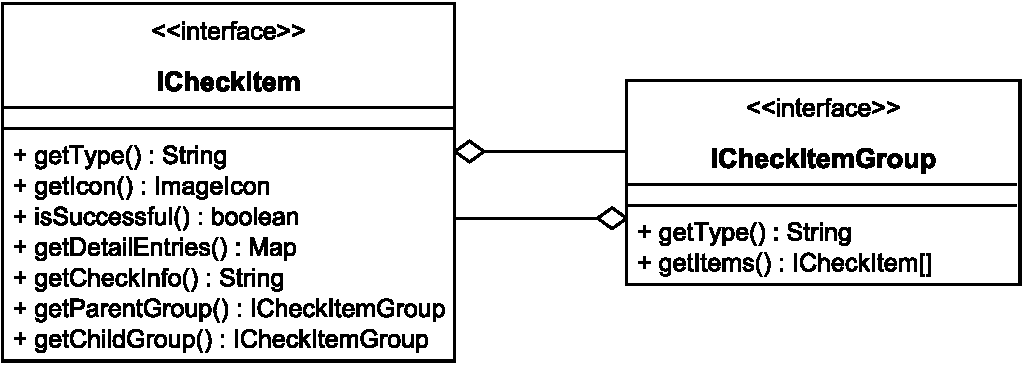
\includegraphics[width=280px]{../graphic/diagrams/CD_Baumstruktur_Results/Baumstruktur}
	\captionsetup{width=235px, justification=raggedleft}
	\caption{Datenmodell für Browsertestergebnisse}
	\label{fig:baumstrukturUML_Results}
\end{figure}

In diesem Modell stellt ein \textbf{ICheckItem} ein einzelnes Testergbnis dar. Eine \textbf{ICheckItemGroup} hält neben einer beliebigen Anzahl von \textbf{ICheckItem}s einen Typ in Form eines \textbf{String}s. Somit kann zu jeder Gruppe die gewünschte Typenbezeichnung hinzugefügt werden. Ein \textbf{ICheckItem} besitzt eine Parent- und ein Childgruppe. Diese können mittels der Methoden \textbf{getParentGroup} und \textbf{getChildGroup} erlangt werden. Über diese Methoden lässt sich durch die Baumstruktur iterieren.

\vspace{-5px}

\subsection{Datenstore}

Damit sowohl die Daten der Entitäten und Aktionen als auch die der Browsertestergebnissen in zuvor geschilderter Form erhalten werden können, soll ein Datenstore zum Einsatz kommen. Dieser liefert die beiden oben beschriebenen Datenmodelle. Dabei kümmert er sich die Daten von anderen Quellen (z.B. XML-Dateien) in die gewünschte Datenmodell-Form zu bringen. Zudem ist er dafür zuständig, die geänderten Daten wieder zurück zu speichern.

Um auch ohne die Integration des ShortcutEditors in den ADTIO Designer testweise Entitäten und deren Aktionen zur Verfügung zu haben, soll ein DummyStore implementiert werden, welcher fiktive Testdaten in die Datenmodelle einfügt.

\vfill

\begin{figure}[H]
	\centering
	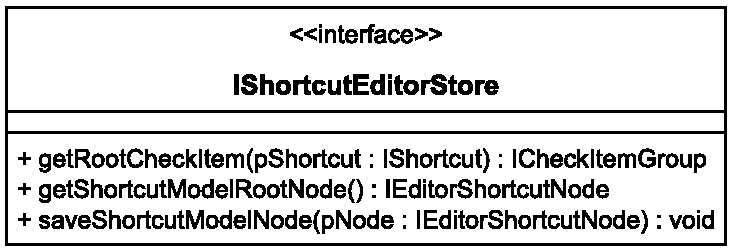
\includegraphics[height=70px]{../graphic/diagrams/CD_IShortcutEditorStore/IShortcutEditorStore}
	\caption{Datenstore}
	\label{fig:ishortcuteditorstore}
\end{figure}



\newpage
\section{Implementierung}

\subsection{Back-End}

\subsubsection{Datenmodelle}

\subsubsection{Datenstore}

\subsection{Front-End}

Nachfolgend wir die Implementierung der GUI beschrieben. Da einige Komponenten schon existiert haben und für den Editor nicht extra

\subsubsection{ShortcutField}

\subsubsection{Accordion}

\newpage

\subsubsection{Check-Button}

Zur Implementierung des im Abschnitt (XXX) erwähnten Check-Buttons wurde zunächst das Interface ICheckComponent erstellt. Indessen wird die Grundfunktionalität einer CheckComponent definiert. Diese besteht darin, dass der Checked-Zustand gesetzt (setChecked(...)) und gelesen (isChecked()) werden kann. Außerdem informiert ein Listener über Änderungen des Zustands. Wird Checked auf true gesetzt, so soll innerhalb der Komponente ein grüner Hacken andernfalls ein rotes Kreuz angezeigt werden. 

Die Klasse CheckToggleButton implementiert das beschriebene Interface und erbt von der Swing Klasse JToggleButton. Sie kümmert sich um das Einfügen und Aktualisieren des richtigen Symbols. Innerhalb von setChecked(...) wird die private Methode \_updateIcon() aufgerufen, welche ihrerseits das jeweilige Symbol über das gesetzte Icon zeichnet (Siehe Anhang (XXX)). Insgesamt stellt ein CheckToggleButton eine vollwertige CheckComponent dar, welche direkt verwendet werden kann.

\begin{figure}[H]
	\centering
	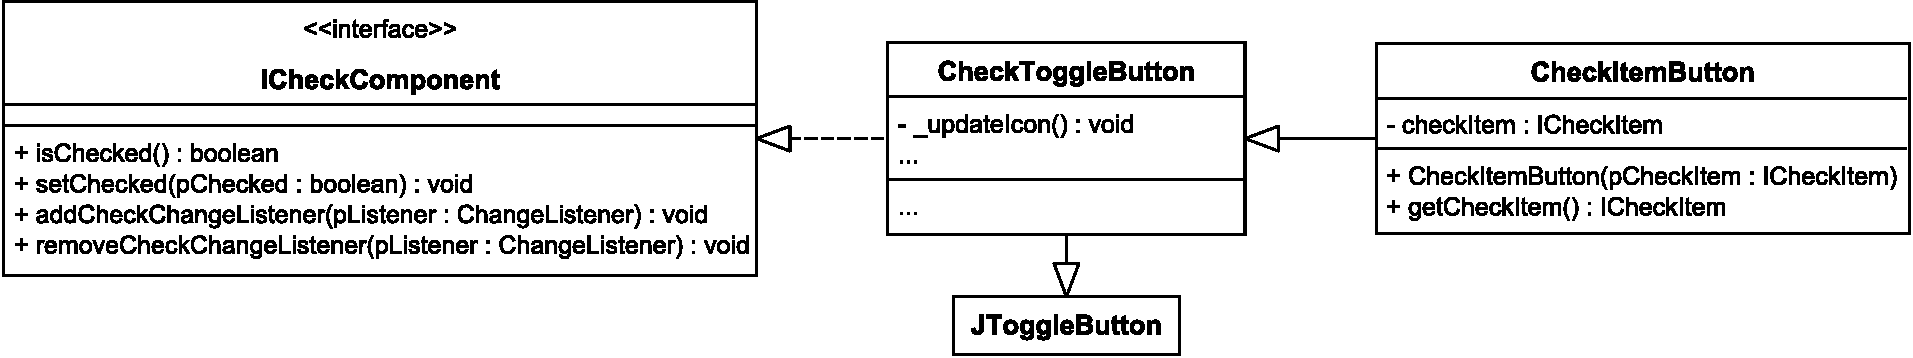
\includegraphics[width=1\linewidth]{../graphic/diagrams/CD_CheckButton/CD_CheckButton}
	\caption{Klassendiagramm des CheckButtons}
	\label{fig:cdcheckbutton}
\end{figure}

Um die Benutzung von CheckToggleButtons innerhalb des Shortcut Editors einfacher zu gestalten, wurde die Klasse CheckItemButton eingeführt, welche CheckToggleButton erweitet und über den Konstruktor ein ICheckItem (siehe (XXX)) aufnehmen kann. Innerhalb dieses Konstruktors werden dem Button alle Eigenschaften entsprechend dem ICheckItem gesetzt (z.B. Checked-Zustand oder Icon).

\subsubsection{CheckItemContainer}

\begin{wrapfigure}[13]{r}[0cm]{160px}
	\vspace{-12px}
	\centering
	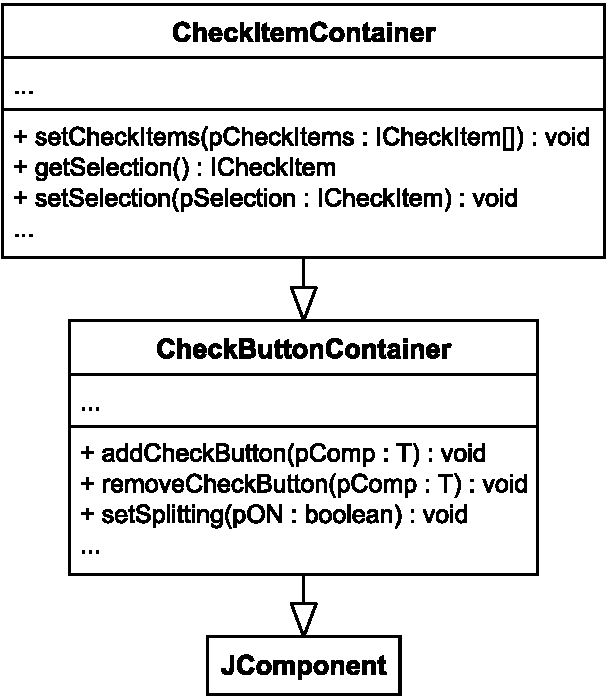
\includegraphics[width=.95\linewidth]{../graphic/diagrams/CD_CheckItemContainer/CD_CheckItemContainer}
	\caption{}
	\label{fig:cdcheckitemcontainer}
\end{wrapfigure}

ewrfqeochwre uow eufoiwqfqjwdeifj iewdj qoew oqwi hequwhe gqweiughqw iuuihqweughfqwueihf  eihwquifh qrhe gfuiqwueihf quih qwihegfuhqwui heuih wqwihe uiqhwueihfquiw hqwheui fhquiwhe fuhweewuhwquei hfhwr fuiqhw 

ewrfqeochwre uow eufoiwqfqjwdeifj iewdj qoew oqwi hequwhe gqweiughqw iuuihqweughfqwueihf  eihwquifh qrhe gfuiqwueihf quih qwihegfuhqwui heuih wqwihe uiqhwueihfquiw hqwheui fhquiwhe fuhweewuhwquei hfhwr fuiqhw 

ewrfqeochwre uow eufoiwqfqjwdeifj iewdj qoew oqwi hequwhe gqweiughqw iuuihqweughfqwueihf  eihwquifh qrhe gfuiqwueihf quih qwihegfuhqwui heuih wqwihe uiqhwueihfquiw hqwheui fhquiwhe fuhweewuhwquei hfhwr fuiqhw 

ewrfqeochwre uow eufoiwqfqjwdeifj iewdj qoew oqwi hequwhe gqweiughqw iuuihqweughfqwueihf  eihwquifh qrhe gfuiqwueihf quih qwihegfuhqwui heuih wqwihe uiqhwueihfquiw hqwheui fhquiwhe fuhweewuhwquei hfhwr fuiqhw 

\newpage
\section{Testphase}

Um sicherzustellen, dass alle implementierten Komponenten anforderungsgerecht funktionieren, wurde der Editor anhand manueller Akzeptanztests getestet. Dabei wurde darauf geachtet, auf jede mögliche Bedienweise einzugehen. So wurde der Editor sowohl per Maus als auch per Tastatur bedient. Gleichzeitig wurde stets überprüft, ob sich der Editor wie gewünscht verhält. Konnte man dabei Unstimmigkeiten feststellen, so wurden die jeweiligen Fehler im Sourcecode behoben und erneut getestet.

Damit die grundlegende Funktionalität auch dauerhaft gewährleistet werden kann, wurde zudem ein automatisierter Test entwickelt (siehe Anhang \ref{Test_ShortcutEditor}). Dabei wurde das Test-Framework \emph{AssertJ Swing} in Kombination mit \emph{JUnit} verwendet.

Das Framework \emph{AssertJ Swing} ist eine Weiterentwicklung des älteren open-source Frameworks \emph{FEST}. Es ermöglicht die einfache Simulation eines Benutzers für Swing Applikationen. Da es als fluent-Api entwickelt wurde, ist der Code sehr gut lesbar und einfach zu verstehen.

Bei \emph{JUnit} handelt es sich ebenfalls um ein quelloffenes Framework, welches durch ein Maven-Plugin in den Build-Vorgang von ADITO eigebunden ist. Dadurch werden alle vorhandenen Tests bei jedem Kompiliervorgang mit Maven automatisch ausgeführt. So können etwaige Fehler schon während der Entwicklung erkannt und vermieden werden.

\begin{wrapfigure}[9]{r}[0px]{322px}
    \centering
	\vspace{-12px}
	\begin{spacing}{0.75}
		\begin{javacode}[firstnumber=28]
@Before
public void onSetUp()
{
  _setLookAndFeel();
  
  dummyStore = new ShortcutDummyStore();
  ui = GuiActionRunner.execute(ShortcutEditorUI::new);
  Dialog shortcutDialog = GuiActionRunner.execute(
      () -> ShortcutEditorDialog.createDialog(dummyStore, ui));
  
  dialog = new DialogFixture(shortcutDialog);
  dialog.show();
}\end{javacode}
	\end{spacing}
	\caption{Setup-Methode}
	\label{fig:Test-ShortcutEditor-onSetUp}
\end{wrapfigure}

In \autoref{fig:Test-ShortcutEditor-onSetUp} ist der Sourcode der Initialisieungsmethode \emph{onSetUp()} dargestellt. Um JUnit anzuweisen, die Methode vor jedem Teststart auszuführen, wurde sie mit der Annotaion \emph{@Before} versehen. 

\vspace{10px}

Nach dem Setzen des ADITO spezifischen Look and Feels, wird der DummyStore und die UI initialisiert. Zum Erstellen des Dialogs werden diese Bestandteile der Methode \emph{ShortcutEditorDialog.createDialog(...)} übergeben. Damit die Ausführung innerhalb des Event Dispatch Threads von Swing erfolgt, kommt ein \emph{GuiActionRunner} zum Einsatz. Dieser führt eine beliebige Anweisung im EDT aus, und liefert das Ergebnis zurück. Nachdem der Dialog erzeugt wurde, wird ein \emph{DialogFixture} erstellt. Hierüber lässt sich der Editor automatisiert bedienen und kann so getestet werden.

\begin{wrapfigure}[11]{l}[0px]{322px}
    \centering
	\vspace{-12px}
	\begin{spacing}{0.75}
		\begin{javacode}[firstnumber=41]
@Test
public void test_EnterShortcut()
{
  int i = 0;
  
  for (IEditorShortcutModel model : dummyStore.getAllModels())
  {
    IShortcut shortcut = new Shortcut(EKeyModifier.SHIFT,
                                      EKey.values()[i++]);
    
    _selectNode(model);
    _enterShortcut(shortcut);
    Assert.assertEquals(model.getShortcut(), shortcut);
  }
}\end{javacode}
	\end{spacing}
	\caption{Test-Methode}
	\label{fig:Test-ShortcutEditor-EnterShortcut}
\end{wrapfigure}

Die mit \emph{@Test} annotierte Testmethode (\autoref{fig:Test-ShortcutEditor-onSetUp}) überprüft, ob eingegebene Shortcuts auch in das selektierte Model übertragen werden. Hierfür wird jedes verfügbare Shortcut Model selektiert und die Eingabe eines Shortcuts simuliert. Der Test ist dann erfolgreich, wenn der Shortcut jedes Models mit dem jeweils zuvor Eingegebenen übereinstimmt.
\newpage
\section{Fazit}

Rückwirkend betrachtet, kann festgehalten werden, dass alle Anforderungen an den Editor gemäß der Projektplanung umgesetzt wurden. Der im Abschnitt (XXX) erwähnte Projektplan konnte eingehalten werden. Die Tabelle in \autoref{fig:sollist} zeigt die tatsächlich benötigten Zeit gegenüber der geplanten. Dabei ist zu erkennen, dass es in den einzelenen Phasen nur zu geringen Zeitabweichungen gekommen ist. Die entstandene Differenzen haben sich untereinander ausgeglichen, wodurch der veranschlagte Zeitrahmen von 70h genau eingehalten werden konnte.

\vfill

\begin{figure}[H] 
	\begin{center}
		\begin{tabularx}{0.90\textwidth}{X|P{50px}|P{50px}|P{50px}}
			\hline \rowcolor{ADITO_RED} \textcolor{white}{\textbf{Vorgang}} & \textcolor{white}{\textbf{Soll}} 								& \textcolor{white}{\textbf{Ist}} 	                            & \textcolor{white}{\textbf{Differenz}} 	\\
			\hline
			1. Analysephase													& 3 h	& 3 h	& 0 h		\\ 
			
			2. Entwurfsphase						 						& 15 h	& 16 h	& + 1 h		\\
			
			3. Implementierungsphase										& 40 h	& 39,5 h& -- 0,5 h	\\
			
			4. Testphase													& 2 h	& 1,5 h	& -- 0,5 h	\\
			5. Dokumentationserstellung										& 10 h 	& 10 h	& 0 h		\\ 
			\hline 
																			& 70 h	& 70 h	& 0 h		\\
		\end{tabularx}
	\end{center}
	\caption{Soll-/Ist-Vergleich} 
	\label{fig:sollist}
\end{figure}

\vfill

Auch das Design konnte wie geplant umgesetzt werden. Vergleicht man den fertigen Editor (\autoref{fig:neuer-editor}) mit dem anfänglich erstellten Designentwurf (\autoref{fig:uxDesigns}) so erkennt man, dass die Anordnung sowie das Aussehen weitestgehend identisch sind.

\vfill

\begin{figure}[H]
	\centering
	\includegraphics[width=1\linewidth]{../graphic/images/screenshots/Neuer-Editor}
	\caption{Screenshot des Editors}
	\label{fig:neuer-editor}
\end{figure}

\vfill

Da der Editor bisher noch nicht in den ADITO Designer integriert ist, sondern in einer eigenen Umgebung gestartet wird, besteht die zukünftige Aufgabe darin, den Editor an den richtigen Stellen des ADITO Designers einzubinden und die Schnittstellen zu entwickeln. Zudem ist es denkbar, dass in Zukunft zusätzliche Anforderungen an den Editor gestellt werden. Beispielsweise könnte es in Zukunft nötig sein, nach gesetzten Shortcuts suchen zu können.

\newpage

\section{Glossar}
\begin{center}
	\begin{tabularx}{\textwidth}{p{.3\textwidth}|X}
	    CRM / xRM & 
		Customer Relationship Management / Any Relationship Management
	  	steht für Kundenpflege/-bindung, Datensammlung, Datenpflege, Datenverwaltung und das Ziel, Kundenpotenziale optimal auszuschöpfen. \\ 
	  	ADITO5 &
	  	ADITO5 ist eine xRM-Lösung, die in Anlehnung an CRM (Customer-Relationship-Management)
	  	zur Verwaltung und Dokumentation aller Arten von Geschäftsbeziehungen dient. \\
	  	ADITO5 Designer &
	  	Der ADITO5 Designer ist die hauseigene Entwicklungsumgebung, mit welcher sowohl die UI als
	  	auch die Businesslogik des Clients entworfen werden kann. \\
	  	Webclient &
	  	Der Webclient ist eine Neuerung von ADITO5, welche mit Hilfe von Vaadin in Java entwickelt wurde. Er stellt eine Web-Applikation dar, welche die gleichen Bedienmöglichkeiten wie der bisherige Client bietet. \\
	  	GUI / UI &
	  	Ein (Grapic) User Interface ist eine grafische Benutzeroberfläche oder auch grafische Benutzerschnittstelle. Sie hat die Aufgabe Anwendungssoftware mittels grafischer Symbole und Steuerelementen bedienbar zu machen. \\
	  	Java Swing &
	  	Swing ist ein GUI-Toolkit von Sun Microsystems. Sie stellt eine Sammlung von Bibliotheken zur Entwicklung grafischer Benutzerschnittstellen. Diese Umfassen Standardkomponenten wie z. B. Buttons, Tabellen oder Textfelder. \\
	  	
	  	Look and Feel &
	  	Das Look and Feel beschreibt das Aussehen und die Handhabung der Software. Dazu gehört beispielsweise die Wahl von Farben, das Layout von grafischen Elementen sowie ihre Reaktion auf Benutzereingaben.
	  	 \\
	\end{tabularx}
\end{center}
\newpage

\section{Abbildungsverzeichnis}
\vspace{-25px}
\renewcommand*\listfigurename{}
\listoffigures
\thispagestyle{fancy}
\section{Literaturverzeichnis}
\begin{itemize}
\item Riehle, Dirk (1996): \glqq Entwurfsmuster\grqq
\end{itemize}
\newpage

\section{Anhang}
\addtocontents{toc}{\protect\setcounter{tocdepth}{-1}}
\subsection{Quellcode}
\subsubsection{TranslateableRemoteLoggerCheckPoint}\label{sec:CODE_TranslateableRemoteLoggerCheckPoint}
\begin{spacing}{0.75}
	\begin{javacode}
/**
 * Erweitert den RemoteLoggerCheckPoint um eine
 * Funktion, diesen zu übersetzen
 *
 * @author W.Glanzer, 19.11.2015
 */
class TranslateableRemoteLoggerCheckPoint extends DefaultRemoteLoggerCheckPoint 
  implements ITranslateableRemoteLoggerCheckPoint
{
  private String translatedMessage;

  /**
   * Wandelt einen CheckPoint in einen RemoteLoggerCheckPoint um
   *
   * @param pCheckPoint CheckPoint, der umgewandelt werden soll
   * @param pTime       Zeit, wann der übergebene CheckPoint aufgetreten ist
   */
  public TranslateableRemoteLoggerCheckPoint(CheckPoint[] pCheckPoint, long pTime)
  {
    super(pCheckPoint, pTime);
    translatedMessage = super.getMessage();
  }
  
  /**
   * Übersetzt den Meldungstext neu, in eine andere Sprache
   *
   * @param pNewLocale gewünschte Lokale, oder <tt>null</tt> für den Systemstandard
   */
  @Override
  public void retranslate(Locale pNewLocale)
  {
    String rc = getResourceCode();
    String[] details = getDetails();
    translatedMessage = Translator.translateCheckpoint(rc, details, pNewLocale);
  }

  @Override
  public String getMessage()
  {
    return translatedMessage;
  }

  @Override
  protected IRemoteLoggerCheckPoint initCause(CheckPoint[] pMyCheckpoint, long pTime)
  {
    CheckPoint[] newTrace = Arrays.copyOfRange(pMyCheckpoint, 1, pMyCheckpoint.length);
    if(pMyCheckpoint.length == 1)
      return null;
      
    return new TranslateableRemoteLoggerCheckPoint(newTrace, pTime);
  }
}  \end{javacode}
\end{spacing}
\newpage

\subsubsection{Implementierungen des Interfaces \glqq IRemoteLoggerCommand\grqq}\label{sec:CODE_IRemoteLoggerCommand}
\begin{figure}[h]
    \centering
    \begin{minipage}{0.5\textwidth}
	    \begin{spacing}{0.75}
		    \begin{javacode}
/**
* Hiermit lässt sich die Sprache einer 
* Verbindung verändern, damit die
* CheckPoints in der vom Client 
* gewählten Sprache ankommen
*
* @author W.Glanzer, 20.11.2015
*/
public class LanguageCommand implements 
	IRemoteLoggerCommand, Serializable
{

  private Locale newLocale;

  public LanguageCommand(Locale pNewLocale)
  {
    newLocale = pNewLocale;
  }

  /**
  * Enthält die neue Sprache, 
  * die der Client möchte
  *
  * @return Die gewünschte Sprache
  */
  public Locale getNewLocale()
  {
    return newLocale;
  }

  @NotNull
  @Override
  public Type getType()
  {
    return Type.LANGUAGE;
  }
}		    \end{javacode}
		\end{spacing}
    \end{minipage}
    \hfill
    \begin{minipage}{0.49\textwidth}
	    \begin{spacing}{0.75}
		    \begin{javacode}
/**
 * Kommando zur Authorisierung eines 
 * Remote-Logger-Clients auf dem
 * Remote-Logger-Server mit bestimmten
 * Login-Informationen
 *
 * @author W.Glanzer, 23.11.2015
 */
public class AuthorizationCommand 
    implements IRemoteLoggerCommand
{

  private String[] loginInformation;

  public AuthorizationCommand(
        String[] pLoginInformation)
  {
    loginInformation = pLoginInformation;
  }

 /**
  * Enthält die LoginInformationen
  *
  * @return Array aus LoginInformationen
  */
  public String[] getLoginInformation()
  {
    return loginInformation;
  }

  @NotNull
  @Override
  public Type getType()
  {
    return Type.AUTHORIZE;
  }
}		    \end{javacode}
	    \end{spacing}
    \end{minipage}
\end{figure}

\subsubsection{ObjectInputStreamConsumer}\label{sec:CODE_ObjectInputStreamConsumer}
\begin{spacing}{0.75}
	\begin{javacode}
/**
 * Kapselt den übergebenen InputStream in einen ObjectInputStream.
 * Dieser liest so lange Daten in einem extra Thread aus,
 * bis ein shutdown angefragt wurde, oder ein Fehler aufgetreten ist
 * und der exceptionHandler einen Retry verweigert hat
 *
 * @author W.Glanzer, 20.11.2015
 */
public class ObjectInputStreamConsumer<Type> implements Runnable
{

  private final InputStream inputStream;
  private final String threadName;
  private final Consumer<Type> objectConsumer;
  private final Function<Exception, Boolean> exceptionHandler;
  private AtomicBoolean shutdownRequested = new AtomicBoolean();

  private ObjectInputStreamConsumer(@NotNull InputStream pInputStream, 
    @Nullable String pThreadName, @NotNull Consumer<Type> pObjectConsumer, 
    @Nullable Function<Exception, Boolean> pExceptionHandler)
  {
    inputStream = pInputStream;
    threadName = pThreadName;
    objectConsumer = pObjectConsumer;
    exceptionHandler = pExceptionHandler;
  }
\end{javacode}
\end{spacing}
\begin{spacing}{0.75}
\begin{javacode}[firstnumber=27]
  /**
   * Erstellt einen ObjectInputStreamConsumer.
   * Dieser liest so lange Daten aus, bis ein shutdown angefragt wurde, oder ein
   * Fehler aufgetreten und der exceptionHandler einen Retry verweigert hat
   *
   * @param pIStream           InputStream, der ausgelesen werden soll. 
   * @param pTName             Name des Threads, in dem der ObjectInputStreamConsumer läuft
   * @param pObjectConsumer    Erhält alle empfangenen Objekte des Consumers
   * @param pExceptionHandler  Erhält alle aufgetretenen Exceptions.
   *                           Wird in dieser Funktion <tt>true</tt> zurückgegeben, dann 
   *                           wird versucht, erneut vom Stream zu lesen.
   *                           Bei <tt>false</tt> wird versucht, die Verbindung zu trennen. 
   * @return Den zugehörigen ObjectInputStreamConsumer
   */   
  public static <T> ObjectInputStreamConsumer<T> consume(@NotNull InputStream pIStream, 
    @Nullable String pTName, @NotNull Consumer<T> pObjectConsumer, 
    @Nullable Function<Exception, Boolean> pExceptionHandler)
  {
    ObjectInputStreamConsumer<T> consumer = 
      new ObjectInputStreamConsumer<>(pIStream, pTName, pObjectConsumer, pExceptionHandler);
    ThreadPool.getInstance().execute(consumer);
    return consumer;
  }
  @Override
  public void run()
  {
    if(threadName != null)
      Thread.currentThread().setName(threadName);

    while(!shutdownRequested.get())
    {
      Object read;
      try
      {
        while ((read = new ObjectInputStream(inputStream).readObject()) != null)
          && !shutdownRequested.get())
        {
          objectConsumer.accept((Type) read);
        }
      }
      catch (Exception e)
      {
        if(exceptionHandler != null && !shutdownRequested.get())
        {
          if(!exceptionHandler.apply(e)) //Kein Retry gewünscht
          {	
            try
            {
              requestShutdown();
            }
            catch (Exception ex)
            {
              exceptionHandler.apply(ex);
            }
          }

          break;
        }
      }
    }
  }

  /**
   * Frägt an, dass sich der StreamConsumer bitte beenden würde.
   * Der anfängliche InputStream wird geschlossen!
   *
   * @throws AditoIOException IOException wenn ein Fehler aufgetreten ist
   */
  public void requestShutdown() throws AditoIOException
  {
    try
    {
      shutdownRequested.set(true);
      inputStream.close();
    }
    catch(Exception e)
    {
      // Stream konnte nicht geschlossen werden
      throw new AditoIOException(e, 10, 403);
    }
  }
}\end{javacode}
\end{spacing}

\subsubsection{Remote-Logger}
\begin{spacing}{0.75}
	\begin{javacode}
/**
 * Logger, der Checkpoints zu verbunden RemoteLogger-Instanzen senden kann
 *
 * @author W.Glanzer, 18.11.2015
 */
public class RemoteLogger extends AbstractLogger
{
  private IRemoteLoggerConnectionHandler connectionHandler;

  private boolean failed = false;
  private Exception failedEx = null;

  /**
   * Erzeugt einen neuen RemoteLogger
   *
   * @param pPriority                die Priorität des Loggers
   * @param pAddress                 die Addresse des Listeners
   * @param pPort                    der Port des Listeners
   * @param pRemoteLoggerLoginFacade Facade zum einloggen von RemoteLogger-Clients 
   *                                 am RemoteLogger-Server, oder <tt>null</tt> wenn 
   *                                 generell alle Clients erlaubt sind
   */
  public RemoteLogger(char pPriority, String pAddress, int pPort, 
    @Nullable Supplier<IRemoteLoggerLoginFacade> pRemoteLoggerLoginFacade)
  {
    try
    {
      IRemoteLoggerCommandHandlerRegistry commandRegistry = 
        new MapRemoteLoggerCommandHandlerRegistry();
      commandRegistry.addHandler(IRemoteLoggerCommand.Type.AUTHORIZE, 
        new AuthorizationCommandHandler(pRemoteLoggerLoginFacade));
      commandRegistry.addHandler(IRemoteLoggerCommand.Type.LANGUAGE, 
        new LanguageCommandHandler());
        
      RemoteLoggerInstanceManager im = RemoteLoggerInstanceManager.getInstance();
      connectionHandler = im.getConnectionHandler(pAddress, pPort);
      connectionHandler.setCommandRegistry(commandRegistry);
      setPriority(pPriority);
    }
    catch (Exception ex)
    {
      System.err.println("RemoteLogger failed:");
      ex.printStackTrace();

      failed = true;
      failedEx = ex;
    }
  }

  /**
   * Hier kann der Logger einen Selbsttest machen. Schlägt dieser fehl 
   * kann er eine neuen Fehler erzeugen damit andere Logger dies melden können.
   *
   * @return <tt>true</tt> wenn der Logger funktioniert, andernfalls <tt>false</tt>
   */
  public boolean checkFunction()
  {
    // Neuen Wert berechnen
    failed = failed || connectionHandler.hasFailed();

    if (failed)
    {
      AditoException ex = new AditoException(failedEx, 0, 32);
      CPH.checkPoint(ex);
    }

    return !failed;
  }

  /**
   * Loggt einen Checkpoint
   *
   * @param pError der Checkpoint
   * @param pTime  die Zeit, wann er aufgetreten ist
   */
  public void logError(CheckPoint[] pError, long pTime)
  {\end{javacode}
        \end{spacing}
        \begin{spacing}{0.75}
        	\begin{javacode}[firstnumber=78]
    if (earlyBreak(pError))
      return;
    if (failed)
      return;
      
    IRemoteLoggerCheckPoint cp = new TranslateableRemoteLoggerCheckPoint(pError, pTime);
    connectionHandler.writeCheckPoint(cp);
  }

  /**
   * Zerstört diesen Logger
   *
   * @throws AditoException Wird geworfen, wenn dieser Logger
   *                        nicht ordnungsgemäß beendet werden konnte
   */
  public synchronized void destroy() throws AditoException
  {
    super.destroy();
    failed = true;
    RemoteLoggerInstanceManager.getInstance().shutdownRemoteLoggerHandler(connectionHandler);
  }

  /**
   * Erstellt eine String-Repräsentanz des RemoteLoggers
   *
   * @return Lesbarer String
   */
  public String toString()
  {
    return "RemoteLogger [" + priority + "]: " + 
      (connectionHandler == null ? "null" : connectionHandler.getSocketAddress());
  }
}\end{javacode}
\end{spacing}

\subsubsection{Implementierung des Interfaces \glqq IRemoteLoggerLoginFacade\grqq}\label{sec:CODE_RemoteLoggerLoginFacadeImpl}
\begin{spacing}{0.75}
	\begin{javacode}
/**
 * Login-Facade, damit sich der RemoteLogger-Client nur dann wirklich
 * einloggen kann, wenn die Login-Daten stimmen!
 *
 * @author W.Glanzer, 26.11.2015
 */
public class RemoteLoggerLoginFacadeImpl implements IRemoteLoggerLoginFacade
{
  private final SecurityPrefs securityPrefs;
  private final LoginPrefs loginPrefs;
  private final Locale locale;
  private final IUserDirectoryExt userDirectory;

  public RemoteLoggerLoginFacadeImpl(@NotNull SecurityPrefs pSecurityPrefs, 
                                     @NotNull LoginPrefs pLoginPrefs,
                                     @Nullable Locale pLocale, 
                                     IUserDirectoryExt pUserDirectory)
  {
    securityPrefs = pSecurityPrefs;
    loginPrefs = pLoginPrefs;
    locale = pLocale;
    userDirectory = pUserDirectory;
  }

  @Override
  public boolean checkLogin(@NotNull String[] pLoginInformation)
  {
    ManagerLoginUtil.LoginResult result = ManagerLoginUtil.checkLogin(pLoginInformation, 
                                          securityPrefs, loginPrefs, locale, userDirectory);
  
    // Überprüft gleichzeitig, ob der hinter den Login-Informationen liegende Benutzer
    // die passende Rolle besitzt.
    return result.wasOK() && UserUtility.hasRole(result.getUser(), InternalRoles.ADMIN);
  }
}  \end{javacode}
\end{spacing}
\newpage

\subsubsection{Implementierung des Interfaces \glqq IRemoteLoggerConnectionHandler\grqq}\label{sec:CODE_RemoteLoggerConnectionHandler}
\input{CODE/CODE_RemoteLoggerConnectionHandler.tex}
\newpage

\subsubsection{Implementierung des Interfaces \glqq IRemoteLoggerServerConnection\grqq}\label{sec:CODE_RemoteLoggerServerConnection}
\begin{spacing}{0.75}
  \begin{javacode}
/**
 * Eine Instanz des Loggers, gekoppelt mit einem ObjectOutputStream
 * Jede Verbindung hat eine eigene Instanz
 *
 * @author W.Glanzer, 18.11.2015
 */
class DefaultRemoteLoggerServerConnection implements IRemoteLoggerServerConnection
{
  private SocketChannel channel;
  private Locale clientLocale;
  private IRemoteLoggerCommandHandlerRegistry registry;
  private boolean authorized;

  /**
   * Erzeugt eine neue Instanz
   *
   * @param pChannel der Netzwerkchannel der Instanz
   */
  public DefaultRemoteLoggerServerConnection(SocketChannel pChannel)
  {
    channel = pChannel;
    clientLocale = Locale.getDefault(); //Anfangswert
    ObjectInputStreamConsumer.consume(Channels.newInputStream(pChannel), null, 
      this::_handleCommand, this::_handleException);
  }

  /**
   * Loggt einen für den RemoteLogger gekapselten Checkpoint
   *
   * @param pCheckpoint Checkpoint, der aufgetreten ist
   * @return <tt>true</tt> wenn erfolgreich
   */
  @Override
  public boolean writeCheckPoint(IRemoteLoggerCheckPoint pCheckpoint)
  {
    try
    {
      if (channel.isConnected() && pCheckpoint != null)
      {
        // Wenn nötig ab hier übersetzen, da nur die Connection weiß, 
        // welche Sprache die verbundene GUI hat
        if(pCheckpoint instanceof ITranslateableRemoteLoggerCheckPoint)
          ((ITranslateableRemoteLoggerCheckPoint) pCheckpoint).retranslate(clientLocale);

        ByteArrayOutputStream baos = new ByteArrayOutputStream();
        ObjectOutputStream oos = new ObjectOutputStream(baos);
        oos.writeObject(pCheckpoint);
        oos.flush();

        channel.write(ByteBuffer.wrap(baos.toByteArray()));

        return true;
      }
      else
        return false;
    }
    catch (Exception ex)
    {
      // Wird geworfen, wenn die Verbindung wieder getrennt ist
      close();
      return false;
    }
  }

  /**
   * Setzt die CommandRegistry zur Verarbeitung von Kommandos
   *
   * @param pRegistry  Registry, die gesetzt werden soll, oder
   *                   <tt>null</tt> wenn alle Commands ignoriert werden sollen
   */
  @Override
  public void setCommandRegistry(@Nullable IRemoteLoggerCommandHandlerRegistry pRegistry)
  {
    registry = pRegistry;
  }
  \end{javacode}
\end{spacing} 
\begin{spacing}{0.75}
  \begin{javacode}[firstnumber=77]		
  /**
   * Setzt die Locale dieser Verbindung.
   * Jede Connection kann ihre eigene Locale besitzen!
   *
   * @param pLocale  Locale, die gesetzt werden soll und
   *                 die Sprache des Clients angibt
   */
  @Override
  public void setLocale(@NotNull Locale pLocale)
  {
    clientLocale = pLocale;
  }
  		
  @Override
  public void setAuthorized(boolean pAuthorized)
  {
    authorized = pAuthorized;
  }

  /**
   * Beendet die Instanz
   */
  @Override
  public void close()
  {
    try
    {
      if (channel.isConnected())
        channel.close();
    }
    catch (Exception ex)
    {
      System.err.println("DefaultRemoteLoggerServerConnection error[1]:");
      ex.printStackTrace();
    }
  }
} \end{javacode}
\end{spacing}

\vspace{-1px}
\subsubsection{Implementierung des Interfaces \\\glqq IRemoteLoggerCommandHandlerRegistry\grqq}
\begin{spacing}{0.75}
	\begin{javacode}
/**
 * Implementierung einer CommandHandlerRegistry, bei der sich
 * verschiedene CommandHandler einhängen lassen.
 * Die Handler werden in einer Map gespeichert, und beim Aufruf
 * von "shutdown" wieder gelöscht!
 *
 * @author W.Glanzer, 20.11.2015
 * @see IRemoteLoggerCommandHandlerRegistry
 */
class MapRemoteLoggerCommandHandlerRegistry implements IRemoteLoggerCommandHandlerRegistry
{

  private final Map<IRemoteLoggerCommand.Type, 
   IRemoteLoggerCommandHandler<? extends IRemoteLoggerCommand>> handlers = new HashMap<>();

  @Override
  public void addHandler(IRemoteLoggerCommand.Type pType, 
   IRemoteLoggerCommandHandler<? extends IRemoteLoggerCommand> pCommandHandler)
  {
    synchronized (handlers)
    {
      handlers.put(pType, pCommandHandler);
    }
  }

  @Nullable
  @Override
  public IRemoteLoggerCommandHandler getHandler(IRemoteLoggerCommand.Type pCommand)
  {
    synchronized (handlers)
    {
      return handlers.get(pCommand);
    }
  }
}    \end{javacode}
\end{spacing}
\newpage

\subsubsection{Implementierungen des Interfaces \glqq IRemoteLoggerCommandHandler\grqq}
\begin{spacing}{0.75}
	\begin{javacode}
/**
 * Handlet das Kommando zur Autorisierung des RemoteLogger-Clients am RemoteLogger-Server.
 * Wenn die Autorisierung erfolgreich ist, dann wird dies der Verbindung gesetzt.
 * Andernfalls wird die Verbindung SOFORT geschlossen!
 *
 * @author W.Glanzer, 23.11.2015
 * @see AuthorizationCommand
 */
public class AuthorizationCommandHandler implements 
  IRemoteLoggerCommandHandler<AuthorizationCommand>
{

  private Supplier<IRemoteLoggerLoginFacade> loginFacadeSupplier;

  /**
   * Erstellt einen CommandHandler zur Autorisierung vom RemoteLogger-Clients am Server
   *
   * @param pRemoteLoggerLoginFacade Facade zum einloggen von RemoteLogger-Clients am 
   *                                 RemoteLogger-Server, oder <tt>null</tt> wenn 
   *                                 generell alle Clients erlaubt sind
   */
  public AuthorizationCommandHandler(
    @Nullable Supplier<IRemoteLoggerLoginFacade> pRemoteLoggerLoginFacade)
  {
    loginFacadeSupplier = pRemoteLoggerLoginFacade;
  }

  @Override
  public void handle(IRemoteLoggerServerConnection pConnection, AuthorizationCommand pCmd)
  {
    IRemoteLoggerLoginFacade loginFacade = null;
    if(loginFacadeSupplier != null)
      loginFacade = loginFacadeSupplier.get()
    
    boolean loginOK = loginFacade == null || 
                        loginFacade.checkLogin(pCmd.getLoginInformation());
    if (loginOK)
      pConnection.setAuthorized(true);
    else
      pConnection.close();
  }

}\end{javacode}
\end{spacing}
\vspace{15px}
\begin{spacing}{0.75}
	\begin{javacode}
/**
 * Handelt das "Language"-Kommando am Server ab
 * und setzt die neue Sprache der ServerConnection.
 * Somit muss dann nicht der Client die CheckPoints übersetzen,
 * sondern der Server schickt diese schon in der richtigen Sprache.
 *
 * @author W.Glanzer, 20.11.2015
 * @see LanguageCommand
 */
public class LanguageCommandHandler 
  implements IRemoteLoggerCommandHandler<LanguageCommand>
{

  @Override
  public void handle(IRemoteLoggerServerConnection pConnection, LanguageCommand pCommand)
  {
    Locale newLocale = pCommand.getNewLocale();
    if(newLocale != null)
      pConnection.setLocale(newLocale);
  }

}\end{javacode}
\end{spacing}
\newpage

\subsubsection{Implementierung des Interfaces \glqq IRemoteLoggerClientConnection\grqq}
\begin{spacing}{0.75}
	\begin{javacode}
/**
 * Verbindung RemoteLogger
 * Manager->Server
 *
 * @author W.Glanzer, 19.11.2015
 */
public class RemoteLoggerClientConnection implements IRemoteLoggerClientConnection
{
  private final List<IRemoteLoggerListener> loggerListenerList = new ArrayList<>();
  private final String host;
  private final int port;
  private String[] loginInformation;
  private boolean closed = false;
  private Socket clientSocket;
  private ObjectInputStreamConsumer<IRemoteLoggerCheckPoint> streamConsumer;

  public RemoteLoggerClientConnection(String pHost, int pPort, String[] pLoginInformation)
  {
    host = pHost;
    port = pPort;
    loginInformation = pLoginInformation;
  }

  @Override
  public void connect() throws AditoIOException
  {
    if ((clientSocket != null && !clientSocket.isClosed()) || closed)
      return;

    try
    {
      clientSocket = new Socket(host, port);
      streamConsumer = ObjectInputStreamConsumer.consume(clientSocket.getInputStream(), 
        null, this::_fireCheckPointReceived, this::_handleException);

      // Einloggen
      sendCommand(new AuthorizationCommand(loginInformation));

      _fireConnectionStatusChanged(true);
    }
    catch (Exception e)
    {
      throw new AditoIOException(e, 16, 206);
    }
  }

  @Override
  public void close() throws AditoIOException
  {
    try
    {
      if (!closed)
      {
        streamConsumer.requestShutdown(); //schließt den inputStream schon
        closed = true;
        clientSocket = null;
        _fireConnectionStatusChanged(false);
      }
    }
    catch (Exception e)
    {
      throw new AditoIOException(e, 16, 207);
    }
  }

  @Override
  public void sendCommand(@NotNull IRemoteLoggerCommand pCommand) throws AditoIOException
  {
    try
    {
      if (!closed)
      {
        ByteArrayOutputStream outputstream = new ByteArrayOutputStream();
        ObjectOutputStream oos = new ObjectOutputStream(outputstream);
        oos.writeObject(pCommand);
        oos.flush();
        byte[] bytes = outputstream.toByteArray();
        oos.close();\end{javacode}
        \end{spacing}
        \begin{spacing}{0.75}
        	\begin{javacode}[firstnumber=79]
        clientSocket.getOutputStream().write(bytes);
      }
    }
    catch (IOException pE)
    {
      throw new AditoIOException(pE, 16, 208, "type: " + pCommand.getType());
    }
  }

  @Override
  public boolean addListener(IRemoteLoggerListener pListener)
  {
    synchronized (loggerListenerList)
    {
      return loggerListenerList.add(pListener);
    }
  }

  @Override
  public boolean removeListener(@Nullable IRemoteLoggerListener pListener)
  {
    synchronized (loggerListenerList)
    {
      return loggerListenerList.remove(pListener);
    }
  }

  /**
   * Feuert, dass der RemoteLogger einen neuen CheckPoint gebracht hat
   *
   * @param pCheckPoint CheckPoint, den der RemoteLogger gebracht hat, nicht <tt>null</tt>!
   */
  private void _fireCheckPointReceived(@NotNull IRemoteLoggerCheckPoint pCheckPoint)
  {
    synchronized (loggerListenerList)
    {
      for (IRemoteLoggerListener currListener : loggerListenerList)
        currListener.checkPointReceived(pCheckPoint);
    }
  }

  /**
   * Feuert, dass der RemoteLogger seinen Verbindungsstatus geänder hat
   *
   * @param pConnectedNow <tt>true</tt>, wenn der Logger jetzt mit dem am Server verbunden 
   *                      ist, bei <tt>false</tt> hat sich dieser getrennt
   */
  private void _fireConnectionStatusChanged(boolean pConnectedNow)
  {
    synchronized (loggerListenerList)
    {
      for (IRemoteLoggerListener currListener : loggerListenerList)
        currListener.connectionStatusChanged(pConnectedNow);
    }
  }

  /**
   * Wird aufgerufen, wenn im ObjectStreamConsumer eine Fehlermeldung aufgetreten ist
   *
   * @param pException  Exception, die aufgetreten ist
   * @return <tt>true</tt>, wenn aus dem Stream erneut ausgelesen werden soll
   */
  private boolean _handleException(@NotNull Exception pException)
  {
    CPH.checkPoint(pException, 16, 210, CPH.OK_DIALOG);
    _fireConnectionStatusChanged(false);
    return false;
  }
}\end{javacode}
\end{spacing}
\newpage

\subsubsection{Implementierungen des Interfaces \glqq IRemoteLoggerListener\grqq}
Listener innerhalb des ADITO4-Managers zur Anzeige aufgetretener CheckPoints innerhalb der TreeTable:
\begin{spacing}{0.75}
	\begin{javacode}
/**
 * Listener um auf Ausgaben und Meldungen im RemoteLogger zu hören.
 * Fügt diesen dann in die TreeTable des ADTIO4-Managers ein
 */
private class _RemoteLoggerListener implements IRemoteLoggerListener
{
  @Override
  public void checkPointReceived(@NotNull IRemoteLoggerCheckPoint pCheckPoint)
  {
    treeTable.addCheckPoint(pCheckPoint);
  }

  @Override
  public void connectionStatusChanged(boolean pIsConnectedNow)
  {
    SwingUtilities.invokeLater(() -> connectionButton.setSelected(pIsConnectedNow));
  }
}	\end{javacode}
\end{spacing}

\vspace{10px}

Listener innerhalb des IRemoteLoggerClientConnectionManagers, damit dieser aufgetretene CheckPoints an seine eigenen Listener verteilen kann.
\begin{spacing}{0.75}
	\begin{javacode}
/**
 * Listener der Nachrichten von der Connection
 * an alle eingehängten RemoteLogger verteilt
 */
private class _ControllingListener implements IRemoteLoggerListener
{
  @Override
  public void connectionStatusChanged(boolean pIsConnectedNow)
  {
    synchronized (listenerList)
    {
      listenerList.forEach(pLoggerListener -> 
        pLoggerListener.connectionStatusChanged(pIsConnectedNow));
    }
  }
  
  @Override
  public void checkPointReceived(@NotNull IRemoteLoggerCheckPoint pCheckPoint)
  {
    synchronized (listenerList)
    {
      listenerList.forEach(pLoggerListener -> 
        pLoggerListener.checkPointReceived(pCheckPoint));
    }
  }
}\end{javacode}
\end{spacing}

\vspace{10px}

Listener des JUnit-Tests der empfangene CheckPoints in der übergebenen Referenz ablegt.
\begin{spacing}{0.75}
	\begin{javacode}
/**
 * Hört darauf, wann CheckPoints empfangen werden.
 * Diese werden in der übergebenen Referenz gespeichert.
 * Alle Threads, die auf diese Referenz warten werden benachrichtigt
 */
private static class _RemoteListener implements IRemoteLoggerListener
{
  private final AtomicReference<IRemoteLoggerCheckPoint> refToSet;
  
  public _RemoteListener(AtomicReference<IRemoteLoggerCheckPoint> pRefToSet)
  {
    refToSet = pRefToSet;
  }
  
  @Override
  public void checkPointReceived(@NotNull IRemoteLoggerCheckPoint pCheckPoint)
  {\end{javacode}
\end{spacing} 
\begin{spacing}{0.75}
	\begin{javacode}[firstnumber=18]
    synchronized (refToSet)
    {
      refToSet.set(pCheckPoint);
      refToSet.notifyAll();
    }
  }
  
  @Override
  public void connectionStatusChanged(boolean pIsConnectedNow)
  {
  }
} \end{javacode}
\end{spacing} 

\subsubsection{Implementierung des Interfaces \\\glqq IRemoteLoggerClientConnectionManager\grqq}
\begin{spacing}{0.75}
	\begin{javacode}
/**
 * Implementierung eines RemoteLoggerClientConnectionManagers.
 * Dieser dient als Zwischenstelle von außen auf die ClientConnection,
 * damti diese bei Bedarf ausgewechselt werden kann
 *
 * @author W.Glanzer, 20.11.2015
 */
public abstract class AbstractRemoteLoggerClientConnectionManager 
  implements IRemoteLoggerClientConnectionManager
{
  private final List<IRemoteLoggerListener> listenerList = new ArrayList<>();
  private final IRemoteLoggerListener listenerController = new _ControllingListener();
  private IRemoteLoggerClientConnection currentConnection;

  @Override
  public void shutdown() throws AditoIOException
  {
    try
    {
      disconnect();
      synchronized (listenerList)
      {
        listenerList.clear();
      }
    }
    catch(Exception e)
    {
      throw new AditoIOException(e, 16, 203);
    }
  }

  @Override
  public void connect(Locale pLocale) throws AditoIOException
  {
    try
    {
      currentConnection = createConnection();
      if(currentConnection != null)
      {
        currentConnection.addListener(listenerController);
        currentConnection.connect();

        // Sprache einstellen
        currentConnection.sendCommand(new LanguageCommand(pLocale));
      }
    }
    catch(Exception e)
    {
      throw new AditoIOException(e, 16, 204);
    }
  }

  @Override
  public void disconnect() throws AditoIOException
  {
    try
    {
      if (currentConnection != null)
      {\end{javacode}
\end{spacing}
\begin{spacing}{0.75}
	\begin{javacode}[firstnumber=60]
        currentConnection.close();
        currentConnection.removeListener(listenerController);
        currentConnection = null;
      }
    }
    catch (Exception e)
    {
      throw new AditoIOException(e, 16, 205);
    }
  }

  @Override
  public void addListener(IRemoteLoggerListener pLoggerListener)
  {
    synchronized (listenerList)
    {
      listenerList.add(pLoggerListener);
    }
  }

  @Override
  public void removeListener(IRemoteLoggerListener pLoggerListener)
  {
    synchronized (listenerList)
    {
      listenerList.remove(pLoggerListener);
    }
  }

  /**
   * Erstellt die Connection
   *
   * @return Die Connection
   */
  @Nullable
  protected abstract IRemoteLoggerClientConnection createConnection() 
    throws AditoException;

  /**
   * Listener der Nachrichten von der Connection
   * an alle eingehängten RemoteLogger verteilt
   */
  private class _ControllingListener implements IRemoteLoggerListener
  {
    @Override
    public void connectionStatusChanged(boolean pIsConnectedNow)
    {
      synchronized (listenerList)
      {
        listenerList.forEach(pLoggerListener -> 
          pLoggerListener.connectionStatusChanged(pIsConnectedNow));
      }
    }

    @Override
    public void checkPointReceived(@NotNull IRemoteLoggerCheckPoint pCheckPoint)
    {
      synchronized (listenerList)
      {
        listenerList.forEach(pLoggerListener ->
          pLoggerListener.checkPointReceived(pCheckPoint));
      }
    }
  }
}\end{javacode}
\end{spacing}
\newpage

\subsubsection{GUI-Implementierung}
Hauptkomponente für die GUI des Remote-Logger-Clients im ADITO4-Manager
\begin{spacing}{0.75}
	\begin{javacode}
/**
 * Panel des RemoteLogger-Clients im Manager
 *
 * @author W.Glanzer, 19.11.2015
 */
public class RemoteLoggerPanel extends AbstractDetailPanel
{
  private final RemoteLoggerTreeTable treeTable;
  private final RemoteLoggerDetailsPanel detailsPanel;
  private JToggleButton connectionButton;

  public RemoteLoggerPanel(RemoteLoggerNode pNode, SMPrefs pPrefs)
  {
    super(pPrefs);
    treeTable = new RemoteLoggerTreeTable();
    treeTable.setBorder(new CompoundBorder(new EmptyBorder(2, 0, 0, 0), 
                                           treeTable.getBorder()));
    treeTable.getTreeTable().getSelectionModel()
      .addListSelectionListener(new _TreeTableSelectionListener());

    detailsPanel = new RemoteLoggerDetailsPanel();

    final AbstractFoldableSplitpane split = SplitpaneFactory
      .createSplitPane(AbstractFoldableSplitpane.TOP_TO_BOTTOM, treeTable, 
                       detailsPanel, true, true);
    split.setFoldable(IFoldableSplitpane.SECOND_FOLDABLE);
    split.setBorder(null);
    IRemoteLoggerClientConnectionManager connectionManager = pNode.getConnectionManager();
    connectionManager.addListener(new _RemoteLoggerListener());
    add(_createToolBar(connectionManager), BorderLayout.NORTH);
    add(split, BorderLayout.CENTER);
    SwingUtilities.invokeLater(() -> {
      split.setDividerLocation((int) ((split.getPreferredSize().getHeight() / 4) * 1.5));
      split.revalidate();
      split.repaint();
    });
  }

  /**
   * Erstellt die Toolbar, zum Steuern des RemoteLogger-Clients
   *
   * @param pManager  ConnectionManager zum steuern des RL-Clients
   * @return Die Toolbar-Komponente
   */
  private JToolBar _createToolBar(IRemoteLoggerClientConnectionManager pManager)
  {
    JToolBar toolbar = new JToolBar();
    toolbar.setFloatable(false);

    connectionButton = new JToggleButton(Imageloader.getInstance().loadIcon(IIcons.LINK_16))
    connectionButton.setToolTipText(Translator.getString(16, 
      IStaticResources.TEXT_CONNECT_TO_LOGGER, Locale.getDefault()));
    connectionButton.addActionListener(new _ConnectButtonListener(pManager));
    toolbar.add(connectionButton);

    JButton clearOutput = new JButton(Imageloader.getInstance().loadIcon(IIcons.TRASH_16));
    clearOutput.setToolTipText(Translator.getString(16, 
      IStaticResources.TEXT_CLEAR_OUTPUT, Locale.getDefault()));
    clearOutput.addActionListener(pEvent -> treeTable.clear());
    toolbar.add(clearOutput);

    return toolbar;
  }

  @Override
  public TableSorter getSorter()
  {
    return null;
  }

  @Override
  public JXTable getTable()
  {
    return null;
  }\end{javacode}
  \end{spacing}
\begin{spacing}{0.75}
	\begin{javacode}[firstnumber=74]
  /**
   * Implementierung eines ActionListeners der aufgerufen wird,
   * wenn der connectionButton gedrückt wird
   */
  private class _ConnectButtonListener implements ActionListener
  {
    private IRemoteLoggerClientConnectionManager connectionManager;

    public _ConnectButtonListener(IRemoteLoggerClientConnectionManager pConnectionManager)
    {
      connectionManager = pConnectionManager;
    }

    @Override
    public void actionPerformed(ActionEvent e)
    {
      try
      {
        if(e.getSource() instanceof JToggleButton)
        {
          JToggleButton button = (JToggleButton) e.getSource();
          boolean selected = button.isSelected();

          // Wieder auf dem normalzustand setzen, da wir selbst das "selected"-Flag setzen!
          button.setSelected(!selected);

          if (selected)
            connectionManager.connect(Locale.getDefault());
          else
            connectionManager.disconnect();
        }
      }
      catch (Exception ex)
      {
        CPH.checkPoint(ex, 16, 209, CPH.OK_DIALOG);
      }
    }
  }

  /**
   * Listener um auf Ausgaben und Meldungen im RemoteLogger zu hören
   */
  private class _RemoteLoggerListener implements IRemoteLoggerListener
  {
    @Override
    public void checkPointReceived(@NotNull IRemoteLoggerCheckPoint pCheckPoint)
    {
      treeTable.addCheckPoint(pCheckPoint);
    }

    @Override
    public void connectionStatusChanged(boolean pIsConnectedNow)
    {
      SwingUtilities.invokeLater(() -> connectionButton.setSelected(pIsConnectedNow));
    }
  }

  /**
   * Dieser Listener springt an, wenn sich
   * die Selektion innerhalb der TreeTable ändert
   */
  private class _TreeTableSelectionListener implements ListSelectionListener
  {
    @Override
    public void valueChanged(ListSelectionEvent e)
    {
      int selectedRow = treeTable.getTreeTable().getSelectedRow();
      if(selectedRow <= -1)
        detailsPanel.setContent(null);
      else
      {
        Object row = treeTable.getTreeTable().getModel().getValueAt(selectedRow, 0);
        if (row instanceof DefaultMutableTreeNode)
        {
          Object uo = ((DefaultMutableTreeNode) row).getUserObject()
          if (uo instanceof IRemoteLoggerCheckPoint)
            detailsPanel.setContent((IRemoteLoggerCheckPoint) uo);
        }
      }
    }
  }
}	\end{javacode}
\end{spacing}
\newpage
Detail-Panel unterhalb der TreeTable im ADITO4-Manager
\begin{spacing}{0.75}
	\begin{javacode}
/**
 * Stellt eine TextArea dar, die selbst die
 * Detailansicht eines RemoteLoggerCheckPoints
 * darstellen kann. Zeigt bspw den StackTrace eines
 * o.g. CheckPoints an
 *
 * @author W.Glanzer, 27.11.2015
 */
class RemoteLoggerDetailsPanel extends ScrollTextArea
{

  public RemoteLoggerDetailsPanel()
  {
    setBorder(null);
    setOpaque(true);
    setBackground(LfUtil.get().getGuiColors().getTaskpaneContainerColorBright());

    getTextArea().setEditable(false);
    getTextArea().setFocusable(false);
  }

  /**
   * Gibt an, welcher CheckPoint genauer angezeigt werden soll, oder <tt>null</tt>,
   * wenn die TextArea geleert werden soll
   *
   * @param pCheckPoint  CheckPoint der angezeigt werden soll, oder <tt>null</tt>
   */
  public void setContent(@Nullable IRemoteLoggerCheckPoint pCheckPoint)
  {
    String t = _toDisplayString(pCheckPoint != null ? pCheckPoint.getDetails() : null)
    getTextArea().setText(t);
    SwingUtilities.invokeLater(() -> getVerticalScrollBar().setValue(0));
  }

  /**
   * Wandelt ein StringArray in einen normalen String um
   *
   * @param pDetails  Details eines CheckPoints
   * @return Ein String, der das Detail-Array repräsentiert, nicht <tt>null</tt>
   */
  @NotNull
  private String _toDisplayString(String[] pDetails)
  {
    if(pDetails == null)
      return "";

    StringBuilder builder = new StringBuilder();
    for (String currDetail : pDetails)
      builder.append(currDetail).append('\n');
    return builder.toString();
  }
}	\end{javacode}
\end{spacing}

\vspace{10px}
TreeTable, in der die CheckPoints angezeigt werden
\begin{spacing}{0.75}
	\begin{javacode}
/**
 * Anzeige der CheckPoints in einer TreeTable
 *
 * @author W.Glanzer, 23.11.2015
 */
class RemoteLoggerTreeTable extends JPanel
{
  private final SplitsTreeTable treeTable;
  private final RemoteLoggerTableModel model = new RemoteLoggerTableModel();

  public RemoteLoggerTreeTable()
  {
    setLayout(new BorderLayout());
    treeTable = new SplitsTreeTable(DefaultOutlineModel.createOutlineModel(model, model, 
     true, Translator.getString(16, IStaticResources.TEXT_TIMESTAMP, Locale.getDefault())));
    
    treeTable.setRootVisible(false);
    treeTable.setRenderDataProvider(new RemoteLoggerTreeDataProvider());
    treeTable.setSelectionMode(ListSelectionModel.SINGLE_SELECTION);
    treeTable.setDefaultRenderer(IRemoteLoggerCheckPoint.class, 
      new RemoteLoggerTreeTableCheckPointRenderer());\end{javacode}
              \end{spacing}
            \begin{spacing}{0.75}
            	\begin{javacode}[firstnumber=22]
    for (TableColumn currColumn : treeTable.getColumns())
    {
      int currIndex = treeTable.getColumnModel().getColumnIndex(currColumn.getIdentifier());
      if(currIndex == 0)
        currColumn.setPreferredWidth(150);
      else if(currIndex == 1)
        currColumn.setPreferredWidth(90);
      else
        currColumn.setPreferredWidth(300);
    }

    treeTable.addFocusListener(new FocusAdapter()
    {
      @Override
      public void focusLost(FocusEvent e)
      {
        // Beim wechsel des Fokus ist ein behalten der Selektion verwirrend
        treeTable.clearSelection();
      }
    });

    SwingUtilities.invokeLater(() -> {
      add(treeTable.getTableHeader(), BorderLayout.NORTH);
      add(new AutoScrollDownScrollPane(treeTable, true), BorderLayout.CENTER);
    });
  }
  
  /**
   * Fügt dem Model einen CheckPoint hinzu
   *
   * @param pCheckPoint CheckPoint, der hinzugefügt werden soll, nicht
   *                    <tt>null</tt>, da das keinen Sinn machen würde!
   */
  public void addCheckPoint(@NotNull IRemoteLoggerCheckPoint pCheckPoint)
  {
    // Alle derzeit expandierten Pfade merken
    TreePathSupport tpSupport = treeTable.getOutlineModel().getTreePathSupport();
    TreePath[] allExpandeds = tpSupport.getExpandedDescendants(new TreePath(model.getRoot()));

    // derzeit selektierte Zeile speichern
    int selectedRow = treeTable.getSelectedRow();

    // Dem Model einen neuen CheckPoint hinzufügen
    model.addCheckPoint(pCheckPoint);

    // expandierte Pfade wieder expandieren
    for (TreePath currPath : allExpandeds)
      tpSupport.expandPath(currPath);

    // selektiert die davor gespeicherte Zeile wieder
    if(selectedRow > -1)
      treeTable.setRowSelectionInterval(selectedRow, selectedRow);

    SwingUtilities.invokeLater(() -> {
      revalidate();
      repaint();
    });
  }

  /**
   * Leert das Ausgabefenster
   */
  public void clear()
  {
    model.clear();

    SwingUtilities.invokeLater(() -> {
      treeTable.revalidate();
      treeTable.repaint();
      revalidate();
      repaint();
    });
  }

  /**
   * @return Die konkrete Instanz der dahinterliegenden TreeTable
   */
  public SplitsTreeTable getTreeTable()
  {
    return treeTable;
  }
}\end{javacode}
\end{spacing}

Model, das die Daten für die Tabelle der o.g. TreeTable liefert
\begin{spacing}{0.75}
	\begin{javacode}
/**
 * Model der RemoteLoggerTreeTable, zur Visualisierung von CheckPoints.
 * Stellt das Model der rechts-liegenden Tabelle dar (2. Teil der TreeTable)
 *
 * @see RemoteLoggerTreeDataProvider
 * @see RemoteLoggerTreeTable
 * @author W.Glanzer, 24.11.2015
 */
class RemoteLoggerTableModel extends DefaultTreeModel implements RowModel
{
  private final DefaultMutableTreeNode rootNode = new DefaultMutableTreeNode();

  public RemoteLoggerTableModel()
  {
    super(null);
    setRoot(rootNode);
  }

  /**
   * Fügt einen CheckPoint in das Model ein und lädt das Model neu
   *
   * @param pCheckPoint CheckPoint, der hinzugefügt werden soll, nicht <tt>null</tt>!
   */
  public void addCheckPoint(@NotNull IRemoteLoggerCheckPoint pCheckPoint)
  {
    rootNode.add(_toNode(pCheckPoint));
    reload(rootNode);
  }

  @Override
  public int getColumnCount()
  {
    return 2; //+1 Tree-Spalte
  }

  @Override
  public Object getValueFor(Object node, int column)
  {
    return node;
  }

  @Override
  public Class getColumnClass(int column)
  {
    return IRemoteLoggerCheckPoint.class;
  }

  @Override
  public boolean isCellEditable(Object node, int column)
  {
    // Generell keine Editiermöglichkeit erlaubt!
    return false;
  }

  @Override
  public void setValueFor(Object node, int column, Object value)
  {
    // Generell keine Editiermöglichkeit erlaubt!
  }

  @Override
  public String getColumnName(int column)
  {
    switch(column)
    {
      case 0:
        return Translator.getString(16, IStaticResources.TEXT_IDENTIFICATION, 
                                     Locale.getDefault());

      case 1:
        return Translator.getString(16, IStaticResources.TEXT_MESSAGE, 
                                     Locale.getDefault());

      default:
        return null;
    }
  }\end{javacode}
                \end{spacing}
              \begin{spacing}{0.75}
              	\begin{javacode}[firstnumber=78]
  /**
   * Leert alle Einträge in der RootNode --> Keine LogAusgaben mehr angezeigt
   */
  public void clear()
  {
    rootNode.removeAllChildren();
    reload(rootNode);
  }

  /**
   * Wandelt einen CheckPoint in eine darstellbare TreeNode um
   *
   * @param pCheckPoint  CheckPoint, der umgewandelt werden soll
   * @return TreeNode, die angezeigt werden kann und die Baumstruktur darstellt
   */
  private MutableTreeNode _toNode(IRemoteLoggerCheckPoint pCheckPoint)
  {
    DefaultMutableTreeNode node = new DefaultMutableTreeNode(pCheckPoint);
    if(pCheckPoint.getCause() != null)
      node.add(_toNode(pCheckPoint.getCause()));
    return node;
  }

}\end{javacode}
\end{spacing}

\vspace{10px}
Modell, das die Daten für den Baum der o.g. TreeTable liefert
\begin{spacing}{0.75}
	\begin{javacode}
/**
 * Stellt die Daten für den Tree der TreeTable bereit
 *
 * @author W.Glanzer, 24.11.2015
 */
class RemoteLoggerTreeDataProvider implements RenderDataProvider
{

  @Override
  public String getDisplayName(Object pNode)
  {
    IRemoteLoggerCheckPoint checkPoint = _toCP(pNode);
    if(checkPoint != null)
      return DateUtility.dateToISO8601(new Date(checkPoint.getTime()), DateUtility.UTC);

    return String.valueOf(pNode);
  }

  @Override
  public String getTooltipText(Object pNode)
  {
    return null;
  }

  @Override
  public boolean isHtmlDisplayName(Object pNode)
  {
    return false;
  }

  @Override
  public Color getBackground(Object pNode)
  {
    return null;
  }
  
  @Override
  public Color getForeground(Object pNode)
  {
    IRemoteLoggerCheckPoint checkPoint = _toCP(pNode);
    if(checkPoint != null)
    {
      IGuiColors colors = LfUtil.get().getGuiColors();
      return CheckPointUtility.getColor(checkPoint.getPriority(), colors.getErrorColor(),
        colors.getWarningColor(), colors.getInfoColor());
    }

    return null;
  }\end{javacode}
    \end{spacing}
  \begin{spacing}{0.75}
  	\begin{javacode}
  @Override
  public Icon getIcon(Object pNode)
  {
    // Kein Icon, auch kein standardicon!
    return new EmptyIcon(0, 0);
  }

  /**
   * Wandelt ein Object in einen RemoteLoggerCheckPoint um, wenn dies funktioniert
   *
   * @param pNode  Object, das umgewandelt werden soll
   * @return Einen RemoteLoggerCheckPoint, oder <tt>null</tt>, wenn es nicht möglich war
   */
  private IRemoteLoggerCheckPoint _toCP(Object pNode)
  {
    if(pNode instanceof DefaultMutableTreeNode)
    {
      Object obj = ((DefaultMutableTreeNode) pNode).getUserObject();
      if (obj instanceof IRemoteLoggerCheckPoint)
        return (IRemoteLoggerCheckPoint) obj;
    }

    return null;
  }
}\end{javacode}
\end{spacing}

\vspace{10px}
Rendert die CheckPoints innerhalb der o.g. TreeTable
\begin{spacing}{0.75}
	\begin{javacode}
/**
 * Rendert einen CheckPoint in der TreeTable (rechten Tabelle)
 *
 * @author W.Glanzer, 24.11.2015
 */
class RemoteLoggerTreeTableCheckPointRenderer extends DefaultOutlineCellRenderer
{

  @Override
  public Component getTableCellRendererComponent(JTable pTable, Object pValue, 
    boolean pIsSelected, boolean pHasFocus, int pRow, int pColumn)
  {
    super.getTableCellRendererComponent(pTable, pValue, pIsSelected, false, pRow, pColumn);
    if(pValue instanceof DefaultMutableTreeNode && 
      ((DefaultMutableTreeNode) pValue).getUserObject() instanceof IRemoteLoggerCheckPoint)
    {
      DefaultMutableTreeNode dmtn = (DefaultMutableTreeNode) pValue
      IRemoteLoggerCheckPoint checkPoint = (IRemoteLoggerCheckPoint) dmtn.getUserObject();

      // Sonst würde die weiße Vordergrundfarbe überschrieben 
      // --> Schlecht leesbar, wenn selektiert
      if(!pIsSelected)
      {
        IGuiColors colors = LfUtil.get().getGuiColors();
        setForeground(CheckPointUtility.getColor(checkPoint.getPriority(), 
          colors.getErrorColor(), colors.getWarningColor(), colors.getInfoColor()));
      }

      switch (pColumn)
      {
        case 1:
          setText(_getID(checkPoint));
          break;

        case 2:
          setText(_getMessage(checkPoint));
          break;
      }
    }

    return this;
  } \end{javacode}
\end{spacing}
\begin{spacing}{0.75}
  	\begin{javacode}
  /**
   * Liefert den Identifier des CheckPoints
   *
   * @param pCheckPoint  CheckPoint, dessen ID gesucht ist
   * @return ID als String
   */
  private String _getID(IRemoteLoggerCheckPoint pCheckPoint)
  {
    return CheckPointUtility.getErrorCode(pCheckPoint.getKind(), pCheckPoint.getModule(),
      pCheckPoint.getPriority(), pCheckPoint.getID(), pCheckPoint.getProgram());
  }

  /**
   * Liefert die zusammengesetzte Nachricht des CheckPoints.
   * Diese setzt sich aus der originalen Message und der Details zusammen
   *
   * @param pCheckPoint  CheckPoint, dessen Nachricht ausgelesen werden soll
   * @return Message + Details als einzelner String
   */
  private String _getMessage(IRemoteLoggerCheckPoint pCheckPoint)
  {
    return pCheckPoint.getMessage();
  }

}	\end{javacode}
\end{spacing}

\subsubsection{Test mit JUnit}
\begin{spacing}{0.75}
	\begin{javacode}
/**
 * Testet den RemoteLogger auf Funktionsfähigkeit
 *
 * @author W.Glanzer, 04.12.2015
 */
public class Test_RemoteLogger
{
  private RemoteLogger logger;
  private final AtomicReference<IRemoteLoggerCheckPoint> lastCheckPointGER = 
    new AtomicReference<>();
  private final AtomicReference<IRemoteLoggerCheckPoint> lastCheckPointENG = 
    new AtomicReference<>();

  /**
   * Initialisiert den Test.
   * Baut den RemoteLogger (localhost, 7733) und den CheckPointHandler auf, damit
   * diese verwendet werden können.
   */
  @Before
  public void init() throws Exception
  {
    logger = new RemoteLogger('Z', "localhost", 7733, _DummyFacade::new);
    CheckPointHandler cph = CPH.init('Z', logger);
    Assert.assertNotNull(cph);
  }

  /**
   * Testet, ob der Remote-Logger einwandfrei funktioniert.
   * Dafür werden zwei Remote-Logger-Clients erzeugt. Diesen werden zwei getrennte Listener
   * eingehangen, die ihre Werte in die jeweils übergebene Referenz speichern.
   * Auf diese Werte wird in dieser Methode gewartet und anschließend verglichen,
   * ob die Werte in deutscher und in englischer Sprache vorhanden und korrekt sind.
   */
  @Test
  public void test_communication() throws Exception
  {
    IRemoteLoggerClientConnectionManager manager = _startClient(Locale.GERMAN);
    IRemoteLoggerClientConnectionManager manager2 = _startClient(Locale.ENGLISH);
    Assert.assertNotNull(manager);
    Assert.assertNotNull(manager2);

    manager.addListener(new _RemoteListener(lastCheckPointGER));
    manager2.addListener(new _RemoteListener(lastCheckPointENG));

    CPH.checkPoint(99, 9999);
    Assert.assertEquals(_getNextCheckPoint(lastCheckPointGER).getID(), 9999);
    Assert.assertEquals(_getNextCheckPoint(lastCheckPointENG).getID(), 9999);\end{javacode}
      \end{spacing}
    \begin{spacing}{0.75}
    	\begin{javacode}[firstnumber=48]
    CPH.checkPoint(0, 1);
    IRemoteLoggerCheckPoint cp = _getNextCheckPoint(lastCheckPointGER);
    Assert.assertEquals(cp.getModule(), 0);
    Assert.assertEquals(cp.getID(), 1);
    Assert.assertEquals(cp.getMessage(), "Interner Fehler. Bitte kontaktieren Sie 
                         Ihren Administrator.");
    Assert.assertEquals(cp.getProgram(), 'Z');
    Assert.assertEquals(cp.getKind(), 'B');
    Assert.assertEquals(cp.getPriority(), 'D');
    Assert.assertTrue(cp.getTime() > 0);
    Assert.assertTrue(cp.getTime() <= System.currentTimeMillis());

    cp = _getNextCheckPoint(lastCheckPointENG);
    Assert.assertEquals(cp.getModule(), 0);
    Assert.assertEquals(cp.getID(), 1);
    Assert.assertEquals(cp.getMessage(), "Internal error. Please contact administrator.");
    Assert.assertEquals(cp.getProgram(), 'Z');
    Assert.assertEquals(cp.getKind(), 'B');
    Assert.assertEquals(cp.getPriority(), 'D');
    Assert.assertTrue(cp.getTime() > 0);
    Assert.assertTrue(cp.getTime() <= System.currentTimeMillis());
  }

  /**
   * Beendet den Test und fährt den Logger herunter.
   * Dieser gibt dann seinen Socket wieder frei
   */
  @After
  public void shutdown() throws Exception
  {
    logger.destroy();
    Assert.assertTrue(true);
  }
  
  /**
   * Blockiert so lange, bis ein neuer CheckPoint eingetroffen ist
   *
   * @param pRefToWaitOn Referenz, in der ein neuer CheckPoint gespeichert wird
   * @return Der empfangene CheckPoint
   */
  @NotNull
  private IRemoteLoggerCheckPoint _getNextCheckPoint(final 
    AtomicReference<IRemoteLoggerCheckPoint> pRefToWaitOn)
  {
    if(pRefToWaitOn.get() == null)
    {
      synchronized (pRefToWaitOn)
      {
        try
        {
          pRefToWaitOn.wait();
        }
        catch (InterruptedException ignored)
        {
        }
      }
    }

    IRemoteLoggerCheckPoint cp = pRefToWaitOn.getAndSet(null);
    Assert.assertNotNull(cp);
    return cp;
  }

  /**
   * Startet einen neuen ConnectionManager, verbindet sich
   * mit dem Server mit einer angegebenen Lokale und gibt diesen
   * Manager dann zurück
   *
   * @return Manager-Instanz der Verbindung
   */
  @Nullable
  private static IRemoteLoggerClientConnectionManager _startClient(Locale pLocale) 
    throws AditoIOException
  {
    _ConnectionManager manager = new _ConnectionManager();
    manager.connect(pLocale);
    return manager;
  }\end{javacode}
        \end{spacing}
      \begin{spacing}{0.75}
      	\begin{javacode}[firstnumber=126]
  /**
   * Implementierung einer LoginFacade, die die
   * LoginInformationen "USER"-"PASS" erwartet.
   * Dadurch lässt sich die Login-Funktionalität prüfen!
   */
  private static class _DummyFacade implements IRemoteLoggerLoginFacade
  {
    @Override
    public boolean checkLogin(String[] pLoginInformation)
    {
      return pLoginInformation.length == 2 &&
          pLoginInformation[0].equals("USER") &&
          pLoginInformation[1].equals("PASS");
    }
  }

  /**
   * Implementiert einen ConnectionManager, der sich auf
   * den Remote-Logger dieses Testes verbindet
   */
  private static class _ConnectionManager 
    extends AbstractRemoteLoggerClientConnectionManager
  {
    @Nullable
    @Override
    protected IRemoteLoggerClientConnection createConnection() throws AditoException
    {
      String[] login = new String[]{"USER", "PASS"};
      return new RemoteLoggerClientConnection("localhost", 7733, login);
    }
  }

  /**
   * Hört darauf, wann CheckPoints empfangen werden.
   * Diese werden in der übergebenen Referenz gespeichert.
   * Alle Threads, die auf diese Referenz warten werden benachrichtigt
   */
  private static class _RemoteListener implements IRemoteLoggerListener
  {
    private final AtomicReference<IRemoteLoggerCheckPoint> refToSet;

    public _RemoteListener(AtomicReference<IRemoteLoggerCheckPoint> pRefToSet)
    {
      refToSet = pRefToSet;
    }

    @Override
    public void checkPointReceived(@NotNull IRemoteLoggerCheckPoint pCheckPoint)
    {
      synchronized (refToSet)
      {
        refToSet.set(pCheckPoint);
        refToSet.notifyAll();
      }
    }

    @Override
    public void connectionStatusChanged(boolean pIsConnectedNow)
    {
    }
  }
}\end{javacode}
\end{spacing}

\end{document}